\documentclass[12pt]{article}

\usepackage[utf8]{inputenc}
\usepackage[T1]{fontenc}
\usepackage{libertine}
\usepackage{libertinust1math}
\usepackage{sourcecodepro}

\usepackage{microtype}

\usepackage[english]{babel}
\usepackage{csquotes}

\usepackage[top=1in, bottom=1.25in, left=1.25in, right=1.25in]{geometry}

\usepackage{booktabs}

\usepackage{graphicx}

\usepackage{solarized-light}
\lstset{%
  basicstyle = \ttfamily\footnotesize, 
  numbers    = left, 
  language   = python,
  aboveskip  = 20pt,
  belowskip  = 20pt
}

\usepackage{hyperref}
\usepackage{xcolor-solarized}

\hypersetup{%
  linkcolor  = solarized-blue,
  citecolor  = solarized-blue,
  urlcolor   = solarized-blue,
  colorlinks = true
}

\renewcommand{\UrlFont}{\normalsize}

% Personal LaTeX styles, see github.com/sdiebolt/latex-styles.
\usepackage{basicmaths}

\begin{document}
  \pagenumbering{Alph}
  \begin{titlepage}
    \begin{center}
      \vspace*{1cm}
 
      \Huge
      \textbf{Machine Learning Module}
 
      \vspace{0.5cm}
      \LARGE
      Homework Report
 
      \vspace{1.5cm}
 
      \textbf{Samuel Diebolt}
 
      \vfill
 
      \vspace{0.8cm}

      
\includegraphics[width=0.8\textwidth]{espci_logo}
 
      \Large
      \textbf{Teacher:} Olivier Rivoire
    \end{center}
    \thispagestyle{empty}
  \end{titlepage}
  \pagenumbering{arabic}

  \section{Course questions}

  \subsection{Maximum likelihood estimation}

  \begin{displayquote}
    \itshape{}
    Alice throws a coin 100 times and obtains 55 times a tail. Estimate by
    maximum likelihood the probability that the coin gives a tails. What
    confidence do we have in this result? Should Alice consider the coin to be
    unfair?
  \end{displayquote}

  We're modelling the outcome of a coin flip by a Bernoulli distribution 
  \begin{equation}
    p_{\text{model}}(x; \theta) = \theta^x {(1 - \theta)}^{1 - x},
  \end{equation} 
  where the parameter $\theta$ represents the probability of getting a tails.
  Thus, the maximum likelihood estimator for $\theta$ is
  \begin{equation}
    \begin{split}
      \theta_{\text{ML}} &= \argmax_\theta \E_{x \sim
        \hat{p}_{\text{data}}} [\log p_{\text{model}}(x; \theta)]\\
      &= \argmax_\theta \left(\hat{\theta} \log\theta + (1 -
        \hat{\theta}) \log(1 - \theta)\right)\\
      &= \hat{\theta},
    \end{split}
  \end{equation}
  where $\hat{\theta}$ is the sample estimate of the probability that the
  coin gives a tails and $\hat{p}_{\text{data}}$ is the empirical
  distribution defined by the observed sample.

  Given that after 100 throws, Alice obtained 55 tails, then
  \begin{equation}
    \theta_{\text{ML}} = \hat{\theta} = 0.55.
  \end{equation}

  Knowing that 
  \begin{equation}
    \begin{split}
      \SE(\theta_{\text{ML}}) &= \sqrt{\frac{\hat{\theta} (1 -
        \hat{\theta})}{n}}\\
      &\approx 0.05
    \end{split}
  \end{equation}
  and considering the normal assumption ($100 \times 0.55 > 30$), the 95\%
  confidence interval is given by
  \begin{equation}
    \theta_{\text{ML}} \in \theta_{\text{ML}} \pm 1.96\times
      \SE(\theta_{\text{ML}}) \approx [0.45, 0.65].
  \end{equation}

  Therefore, as the 95\% confidence interval contains 0.5, Alice cannot reject
  the null hypothesis that her coin is fair (at the 5\% confidence level).
  
  \subsection{Bayesian estimation}

  \begin{displayquote}
    \itshape{}
    Bob is tested for a disease. The test, which is either positive or
    negative, is only 90\% reliable. Given that 1\% of people of Bob’s age and
    background have the disease, what is the probability that Bob has the
    disease?
  \end{displayquote}

  Since we know nothing about the test results, we will assume that the test
  came back positive (without this assumption, the only valid conclusion would
  be that Bob has a 1\% probability of having the disease).

  Considering the events 
  \begin{itemize}
    \item \textbf{ill}: ``Bob has the disease'',
    \item \textbf{+}: ``Bob has tested positive'',
  \end{itemize}
  and given that 
  \begin{equation}
    \begin{cases}
      P(+ | \text{ill}) = 0.90,\\
      P(\text{ill}) = 0.01,
    \end{cases}
  \end{equation}
  then using Bayes' theorem,
  \begin{equation}
    \begin{split}
      P(\text{ill} | +) &= \frac{P(\text{ill}, +)}{P(+)}\\
      &= \frac{P(+ | \text{ill}) P(\text{ill})}{P(+ | \text{ill})P(\text{ill})
        + P(+ | \overline{\text{ill}})P(\overline{\text{ill}})}\\
      &= \frac{0.90 \times 0.01}{0.90 \times 0.01 + 0.10 \times 0.99}\\
      &\approx 0.08.
    \end{split}
  \end{equation}

  Thus, given that Bob has tested positive, he has a probability of about 8\%
  to have the disease. This low probability reflects the lack of information we
  have (in fact, in a medical environment, the test result would be called
  *reactive* instead of *positive* and further testing would be done).
  Obvisouly, other factors (contact with contagious people, etc.), if taken
  into account in a refined model, could help Bob know if the result was a
  false or a true positive.

  For example, a second positive test, given that the prior $P(\text{ill})$ has
  been updated to 8\%, would give a probability of about 44\% that Bob has the
  disease. A third positive test would increase this probability to 88\%.

  \begin{displayquote}
    \itshape{}
    By redesigning the test, you can either reduce from 10\% to 5\% the false
    positive rate (less negative results when the patient is positive) or
    reduce from 10\% to 5\% the false negative rate (less positive results when
    the patient is negative): what is preferable?
  \end{displayquote}

  In the field of disease testing, false negatives are usually considered worse
  than false positives. Taking COVID-19 as an example: a false positive would
  lead to a heavy mental burden for the patient, but further testing would
  eventually show that they aren't ill, while a false negative would mean that
  the patient would be missing out on crucial treatments and runs a risk of
  spreading the disease. Therefore, decreasing the false negative rate is
  preferable for this test.

  \subsection{Information theory}

  \begin{displayquote}
    \itshape{}
    The binary erasure channel is a discrete memoryless channel where each
    input $x_i \in \{0, 1\}$ is either transmitted reliably, with probability
    $1-\epsilon$, or replaced by an error symbol $\star$, with probability
    $\epsilon$. What is the capacity of this channel?
  \end{displayquote}

  For a binary erasure channel with a probability $\epsilon$ of transmitting an
  error,
  \begin{equation}
    \begin{split}
      I(X; Y) &= H(X) - H(X | Y)\\
      &= H(X) - P(y = 0) H(X | y = 0) - P(y = 1) H(X | y = 1) - P(y = \star) H(X
        | y = \star).
    \end{split}
  \end{equation}

  Given $y \neq \star$, $X$ is entirely determined by $Y$, thus
  \begin{equation}
    H(X | y = 0) = H(X | y = 1) = 0.
  \end{equation}

  Also,
  \begin{equation}
    P(y = \star) = \epsilon
  \end{equation}
  by definition of a binary erasure channel, and
  \begin{equation}
    H(X |y = \star) = H(X)
  \end{equation}
  by symmetry (knowing that $y = \star$ doesn't give any information about $X$,
  so $P(X | y = \star) = P(X)$). Therefore,
  \begin{equation}
    I(X; Y) = (1 - \epsilon)H(X).
  \end{equation}

  Finally, the capacity of a binary erasure channel is
  \begin{equation}
    \begin{split}
      C &= \sup_{p_X} I(X; Y)\\
      &= (1 - \epsilon) \sup_{p_X} H(X)\\
      &= 1 - \epsilon.
    \end{split}
  \end{equation}

  The last equation holds if $X$ comes from a Bernoulli distribution with
  parameter $\frac{1}{2}$, as the symmetry would suggest.

  \begin{displayquote}
    \itshape{}
    More generally, a memoryless erasure channel takes inputs from an alphabet
    of $q$ symbols $\{1, 2, \dots, q\}$: any of these symbols is transmitted
    reliably with probability $1-\epsilon$ and replaced by an error symbol
    $\star$ with probability $\epsilon$. What is the capacity of this channel?
  \end{displayquote}

  A memoryless erasure channel taking inputs from an alphabet of $q$ symbols
  would have the same capacity as a binary erasure channel. This result is
  analogous to the previous proof, where $X$ now comes from a categorical
  distribution (generalized Bernoulli) with parameter $\frac{1}{q}$ and the
  entropy $H_q$ is now computed using a logarithm to base $q$.

  \subsection{Maximum entropy method}

  \begin{displayquote}
    \itshape{}
    Consider $N$ binary sequences of length $p$: $\sigma_{i, j} = \pm 1$ with
    $i = 1, \dots, N$ and $j = 1, \dots , p$. We use the maximum entropy method
    to estimate $P(\sigma_1, \dots, \sigma_p)$. Show that if we choose to
    constrain for each $j$ the average of $\sigma_j$ to the empirical mean
    $\mu_j = \sum_i \frac{\sigma_{i, j}}{N}$, the maximum entropy principle
    leads to a distribution of the form.
    \begin{equation}
      P(\sigma_1, \dots, \sigma_p) = \frac{1}{Z}\exp\left(\sum_{j = 1}^p \beta_j
        \sigma_j\right).
    \end{equation}
  \end{displayquote}

  Let $\bm{\sigma} = (\sigma_1, \dots, \sigma_p)$. The first constraint on the
  unknown probability distribution is that its sum must normalize to 1,
  \begin{equation}
    \sum_{\bm{\sigma}} P(\bm{\sigma}) = 1.
  \end{equation}

  Additionally, the first moment of each variable $\sigma_j$ is supposed to
  match the value of the corresponding sample mean over the $N$ measurements,
  \begin{equation}
    \langle \sigma_j \rangle = \sum_{\sigma\in\{-1, 1\}} P_{\sigma_j}(\sigma)
      \sigma = \frac{1}{N} \sum_{i = 1}^N \sigma_{ij} = \overline{\sigma_j},
  \end{equation}
  where $P_{\sigma_j}$ is the marginal probability distribution of $\sigma_j$.
  Further deriving the first moment,
  \begin{equation}
    \begin{split}
      \langle \sigma_j \rangle &= \sum_{\sigma\in\{-1, 1\}}
        P_{\sigma_j}(\sigma) \sigma\\
      &= \sum_{\bm{\sigma}} P(\bm{\sigma}) \sigma_j.
    \end{split}
  \end{equation}

  Finally, the probability distribution should maximize the information entropy:
  \begin{equation}
    S = -\sum_{\bm{\sigma}} P(\bm{\sigma}) \log P(\bm{\sigma}).
  \end{equation}

  Introducing the frequencies $f_j\equiv \overline{\sigma_j}$, the
  corresponding Lagrangian $\cL = \cL(P(\bm{\sigma}); \alpha,
  \{\beta_j\})$ has the functional form
  \begin{equation}
    \cL = S + \alpha\left(\sum_{\bm{\sigma}} P(\bm{\sigma}) -
      1\right) + \sum_{j = 1}^p \beta_j \left(\sum_{\bm{\sigma}}
      P(\bm{\sigma})\sigma_j - f_j\right)
  \end{equation}
  and its stationary point is found at
  \begin{equation}
    \begin{split}
      &\frac{\partial \cL}{P(\bm{\sigma})} = -\log P(\bm{\sigma}) - 1
        + \alpha + \sum_{j = 1}^p \beta_j \sigma_j = 0\\
      \iff& P(\bm{\sigma}) = \frac{1}{Z}\exp\left(\sum_{j = 1}^p \beta_j
        \sigma_j\right),
    \end{split}
  \end{equation}
  where $Z \equiv e^{1 - \alpha}$ is the partition function introduced as
  normalization constant.

  \begin{displayquote}
    \itshape{}
    What are the values of $\beta_j$ and $Z$?
  \end{displayquote}

  First, let us demonstrate the following identity:
  \begin{equation}\label{eq:identity}
    \sum_{\bm{\sigma}} \exp\left(\sum_{j = 1}^p \beta_j \sigma_j\right) =
      \prod_{j = 1}^p \sum_{\sigma_j\in\{-1, 1\}} \exp(\beta_j \sigma_j).
  \end{equation}

  This comes easily by rewriting the left hand sum,
  \begin{equation}
    \begin{split}
      \sum_{\bm{\sigma}} \exp\left(\sum_{j = 1}^p \beta_j \sigma_j\right) &=
        \sum_{\bm{\sigma}} \prod_{j = 1}^p \exp(\beta_j \sigma_j)\\
      &= \sum_{\sigma_1\in\{-1, 1\}}\cdots \sum_{\sigma_p\in\{-1, 1\}} \prod_{j
        = 1}^p \exp(\beta_j \sigma_j)\\
      &= \left(\sum_{\sigma_1\in\{-1, 1\}} \exp(\beta_1 \sigma_1)\right) \cdots
        \left(\sum_{\sigma_p\in\{-1, 1\}} \exp(\beta_p \sigma_p)\right)\\
      &= \prod_{j = 1}^p \sum_{\sigma_j\in\{-1, 1\}} \exp(\beta_j \sigma_j).
    \end{split}
  \end{equation}

  Now, recall that we required the probability distribution to follow the
  constraints,
  \begin{subnumcases}{}
    \sum_{\bm{\sigma}} P(\bm{\sigma}) = 1,\label{eq:constsingle1}\\
    \sum_{\bm{\sigma}} P(\bm{\sigma}) \sigma_j = f_j, &\text{for } j = 1,
      \dots, p.\label{eq:constsingle2} 
  \end{subnumcases}

  Using identity~\eqref{eq:identity}, equation~\eqref{eq:constsingle1} leads to
  \begin{equation}\label{eq:zsingle}
    \begin{split}
      &\sum_{\bm{\sigma}} P(\bm{\sigma}) = 1\\
      \iff& \sum_{\bm{\sigma}} \frac{1}{Z} \exp\left(\sum_{j = 1}^p \beta_j
        \sigma_j\right) = 1\\
      \iff& \frac{1}{Z} \prod_{j = 1}^p \sum_{\sigma_j\in\{-1, 1\}}
        \exp(\beta_j \sigma_j) = 1\\
        \iff& Z = \prod_{j = 1}^p 2 \cosh \beta_j.
    \end{split}
  \end{equation}

  For $k = 1, \dots, p$, using once again identity~\eqref{eq:identity},
  equation~\eqref{eq:constsingle2} leads to
  \begin{equation}
    \begin{split}
      &\sum_{\bm{\sigma}} P(\bm{\sigma}) \sigma_k = f_k\\
      \iff& \sum_{\bm{\sigma}} \left(\prod_{j = 1}^p\exp(\beta_j
        \sigma_j)\right) \sigma_k = f_k Z\\
      \iff& \left(\prod_{j = 1; j\neq k}^p \sum_{\sigma_j\in\{-1, 1\}}
        \exp(\beta_j \sigma_j)\right) \times \sum_{\sigma_k\in\{-1, 1\}}
        \exp(\beta_k \sigma_k) \sigma_k = f_k Z\\
      \iff& \frac{Z}{2 \cosh(\beta_k)} \times 2 \sinh(\beta_k) = f_k Z\\
      \iff& \beta_k = \tanh^{-1} f_k.
    \end{split}
  \end{equation}

  Therefore, introducing this last result into equation~\eqref{eq:zsingle}
  leads to
  \begin{equation}
    Z = \prod_{j = 1}^p \frac{2}{\sqrt{1 - f_j^2}}.
  \end{equation}

  Finally, these results yield the probability distribution assigned to the $p$
  binary sequences with $\sigma_j\in\{-1, 1\}$,
  \begin{equation}\label{eq:probasingle}
    P(\bm{\sigma}) = \frac{1}{Z}\exp\left(\sum_{j = 1}^p \beta_j
      \sigma_j\right),
  \end{equation}
  where
  \begin{equation}
    \begin{cases}
      \beta_j = \tanh^{-1} f_j,\\[1em]
      Z = \displaystyle\prod_{j = 1}^p \frac{2}{\sqrt{1 - f_j^2}}.
    \end{cases}
  \end{equation}

  \begin{displayquote}
    \itshape{}
    What if we take $\sigma_{i, j} \in \{0, 1\}$ instead of $\sigma_{i, j} \in
    \{-1, 1\}$?
  \end{displayquote}

  If $\sigma_{i, j} \in \{0, 1\}$, only the values of $\beta_j$ and $Z$
  changes. Equation~\eqref{eq:constsingle1} now leads to
  \begin{equation}\label{eq:zsingle2}
    \begin{split}
      &\sum_{\bm{\sigma}} P(\bm{\sigma}) = 1\\
      \iff& \sum_{\bm{\sigma}} \frac{1}{Z} \exp\left(\sum_{j = 1}^p \beta_j
        \sigma_j\right) = 1\\
      \iff& \frac{1}{Z} \prod_{j = 1}^p \sum_{\sigma_j\in\{0, 1\}} \exp(\beta_j
        \sigma_j) = 1\\
      \iff& Z = \prod_{j = 1}^p (1 + \exp\beta_j).
    \end{split}
  \end{equation}

  For $k = 1, \dots, p$, equation~\eqref{eq:constsingle2} now leads to
  \begin{equation}
    \begin{split}
      &\sum_{\bm{\sigma}} P(\bm{\sigma}) \sigma_k = f_k\\
      \iff& \sum_{\bm{\sigma}} \left(\prod_{j = 1}^p\exp(\beta_j
        \sigma_j)\right) \sigma_k = f_k Z\\
      \iff& \left(\prod_{j = 1; j\neq k}^p \sum_{\sigma_j\in\{-1, 1\}}
        \exp(\beta_j \sigma_j)\right) \times \sum_{\sigma_k\in\{0, 1\}}
        \exp(\beta_k \sigma_k) \sigma_k = f_k Z\\
      \iff& \frac{Z}{1 + \exp\beta_k} \times \exp\beta_k = f_k Z\\
      \iff& \beta_k = \log\left(\frac{f_k}{1 - f_k}\right).
    \end{split}
  \end{equation}

  Therefore, introducing this last result into equation~\eqref{eq:zsingle2}
  leads to
  \begin{equation}
    Z = \prod_{j = 1}^p \frac{1}{1 - f_j}.
  \end{equation}

  Finally, for binary sequences with $\sigma_j\in\{0, 1\}$, the probability
  distribution in equation~\eqref{eq:probasingle} now has parameters
  \begin{equation}
    \begin{cases}
      \beta_j = \log\left(\displaystyle\frac{f_j}{1 - f_j}\right),\\[1em]
      Z = \displaystyle\prod_{j = 1}^p \frac{1}{1 - f_j}.
    \end{cases}
  \end{equation}

  It is reassuring to see that this probability distribution can be written as
  \begin{equation}
    P(\bm{\sigma}) = \prod_{j = 1}^p f_j^{\sigma_j} {(1 - f_j)}^{1 -
      \sigma_j},
  \end{equation}
  which is a product of Bernoulli probability distributions with parameter
  $f_j$. These are in fact the marginal probability distributions of the
  $\sigma_j$ variables: this last result could have been derived directly from
  the fact that the $\sigma_j$ are mutually independent.

  \begin{displayquote}
    \itshape{}
    What if we also constrain the pair frequencies $f_{jk}$ at which $\sigma_j
    = 1$ and $\sigma_k = 1$ co-occur for every pair $(j, k)$?
  \end{displayquote}

  The constraints are now
  \begin{subnumcases}{}
    \sum_{\bm{\sigma}} P(\bm{\sigma}) = 1,\\
    \sum_{\bm{\sigma}} P(\bm{\sigma}) \sigma_j = f_j, &\text{for } j = 1,
    \dots, p,\\
    \sum_{\bm{\sigma}} P(\bm{\sigma}) \sigma_j \sigma_k = f_{jk}, &\text{%
        for } j,k = 1, \dots, p,
  \end{subnumcases}
  where we introduced the pairwise frequencies $f_{jk} = \overline{\sigma_j
  \sigma_k}$,
  \begin{equation}
    f_{jk}\equiv \overline{\sigma_j \sigma_k} = \frac{1}{N} \sum_{i = 1}^N
      \sigma_{i, j} \sigma_{i, k}.
  \end{equation}

  The corresponding Lagrangian $\cL = \cL(P(\bm{\sigma});
  \alpha, \{\beta_j\}, \{\gamma_{jk}\})$ has the functional form
  \begin{equation}
    \cL = S + \alpha\left(\sum_{\bm{\sigma}} P(\bm{\sigma}) -
      1\right) + \sum_{j = 1}^p \beta_j \left(\sum_{\bm{\sigma}}
      P(\bm{\sigma})\sigma_j - f_j\right) + \sum_{j,k = 1}^p \gamma_{jk}
      \left(\sum_{\bm{\sigma}} P(\bm{\sigma})\sigma_j \sigma_k - f_{jk}\right)
  \end{equation}
  and its stationary point is found at
  \begin{equation}
    \begin{split}
      &\frac{\partial \cL}{P(\bm{\sigma})} = -\log P(\bm{\sigma}) - 1
        + \alpha + \sum_{j = 1}^p \beta_j \sigma_j + \sum_{j,k = 1}^p \gamma_{jk}
        \sigma_j \sigma_k = 0\\
      \iff& P(\bm{\sigma}) = \frac{1}{Z}\exp\left(\sum_{j = 1}^p \beta_j
        \sigma_j + \sum_{j,k = 1}^p \gamma_{jk} \sigma_j \sigma_k\right),
    \end{split}
  \end{equation}
  where $Z\equiv \exp(1 - \alpha)$ is the partition function.

  \newpage
  \section{Lasso regression and model selection: what makes a good wine?}

  This section will study the qualities of \textit{vinho verde}, a wine from
  the Minho (northwest) region of Portugal. The provided datasets (Cortez
  \textit{et al.}, 2009) are available to download
  \href{http://www3.dsi.uminho.pt/pcortez/wine/}{on the author's website} and
  contain twelve features of a sample of red and white \textit{vinho verde}
  wines, ranging from objective test results (e.g.\ pH values) to sensory data
  (evaluations made by wine experts).

  The goal of this section is to preprocess and use these datasets to
  \begin{itemize}
    \item find a predictive model of red wine quality using lasso regression;
    \item implement a classifier that will be able to recognize red and white
      wines from their physicochemical properties.
  \end{itemize}

  Listing~\ref{lst:libraries} shows the Python libraries and plot rendering
  settings used to run all code blocks in this report.

  \begin{lstlisting}[caption={Python libraries import.}, captionpos=b,
    label={lst:libraries}]
# Python libraries.
from IPython.display import display
import numpy as np
import pandas as pd
import plotly.figure_factory as ff
import plotly.graph_objects as go
import plotly.io as pio
from plotly.subplots import make_subplots
from scipy import stats
from scipy.cluster.hierarchy import linkage
from sklearn.cluster import KMeans
from sklearn.decomposition import PCA
from sklearn.linear_model import lasso_path, Lasso, LassoCV
from sklearn.manifold import TSNE
from sklearn.metrics import classification_report
from sklearn.model_selection import train_test_split 
from sklearn.preprocessing import StandardScaler
from sklearn.svm import LinearSVC
import statsmodels.api as sm

# Set random generator seed.
np.random.seed(42)

# Set up plotly renderer.
png_renderer = pio.renderers["svg"]
png_renderer.width = 900
png_renderer.height = 700

pio.renderers.default = "svg"
  \end{lstlisting}

  \newpage

  \subsection{Preprocessing}

  Figure~\ref{fig:redwineheader} shows the different features available in the
  \lstinline{winequality-red} dataset, displayed using
  Listing~\ref{lst:redwineheader}

  \begin{lstlisting}[caption={Print red wine dataset header.}, captionpos=b,
    label={lst:redwineheader}]
# Read red wine quality dataset and display table head.
red_wine = pd.read_csv("data/winequality/winequality-red.csv", 
                       sep=";")
red_wine.head()
  \end{lstlisting}

  \begin{figure}[!ht]
    \centering
    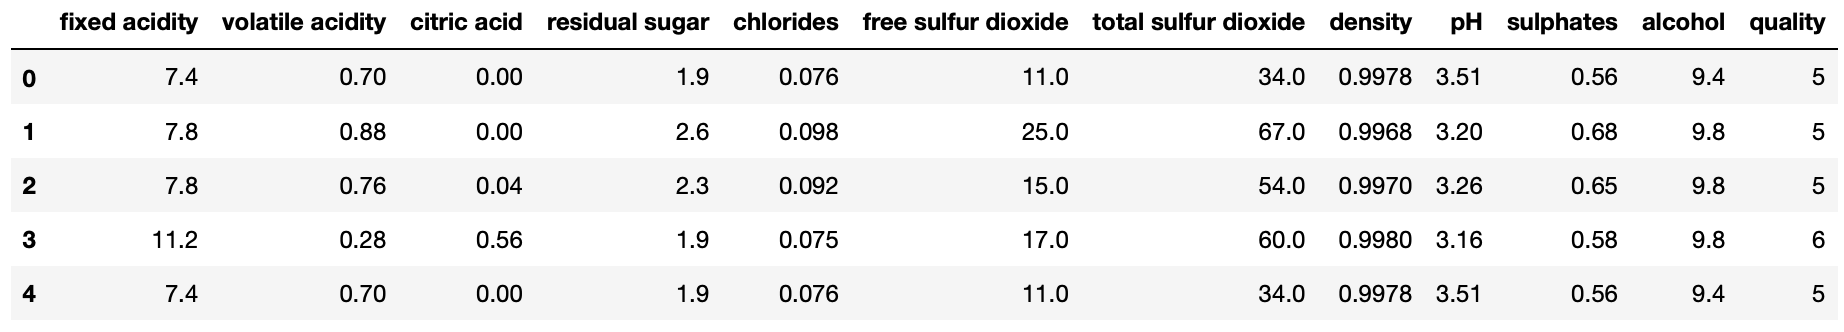
\includegraphics[width=\textwidth]{figures/redwineheader}
    \caption{Red wine quality dataset header.}%
    \label{fig:redwineheader}
  \end{figure} 

  Figure~\ref{fig:redwinehisto1} shows histograms of these features. Some
  features contain outliers that could introduce bias in the following
  analyses: a preprocessing step, performed in Listing~\ref{lst:redwinehisto1},
  will remove values outside the $\pm 3$ standard deviations range.

  \begin{lstlisting}[caption={Preprocessing step.}, captionpos=b,
    label={lst:redwinehisto1}]
# Plot histograms for each variable.
fig = make_subplots(rows=4, cols=3)

for i, col in enumerate(red_wine.columns, 1):
  fig.add_trace(
    go.Histogram(
      x=red_wine[col],
      name=col
    ), 
    row=int(np.ceil(i / 3)), 
    col=i % 3 if i % 3 != 0 else 3
  )

fig.update_layout(
  title_text="Histograms Of Red Wine Features - Before Outlier Removal",
  height=800
)
fig.show() 
  \end{lstlisting}

  \begin{figure}[!ht]
    \centering
    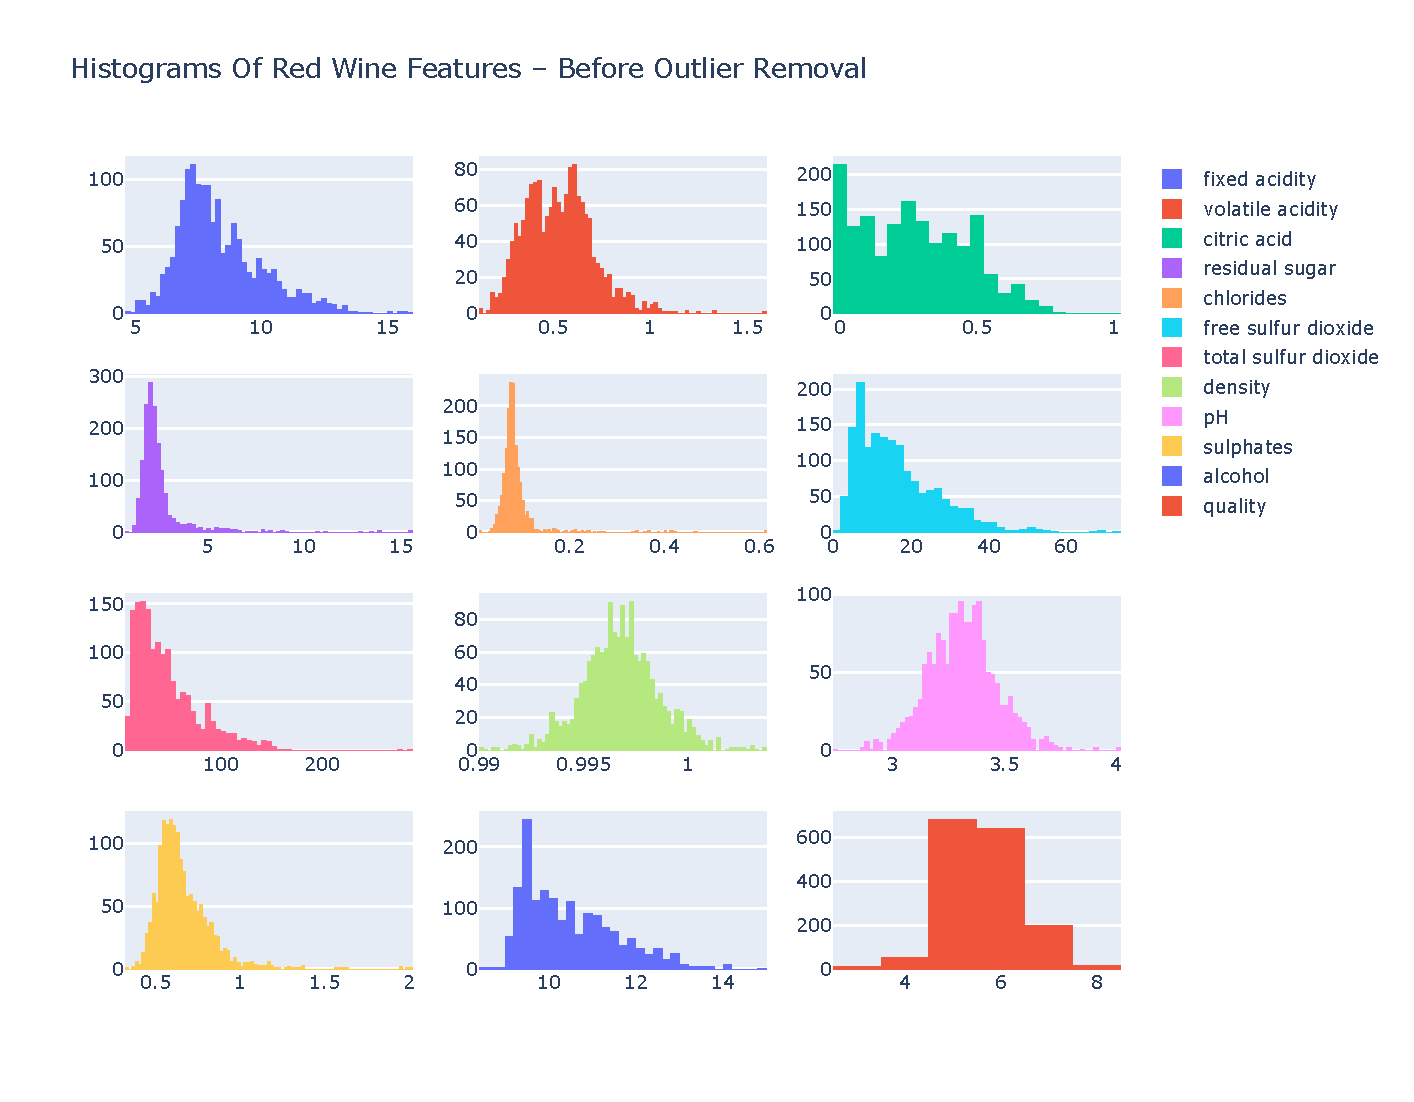
\includegraphics[width=0.75\textwidth]{figures/redwinehisto1}
    \caption{Red wine features histograms before outlier removal.}%
    \label{fig:redwinehisto1}
  \end{figure} 

  Figure~\ref{fig:redwinehisto2} shows the histograms after outlier removal.
  \begin{figure}[!ht]
    \centering
    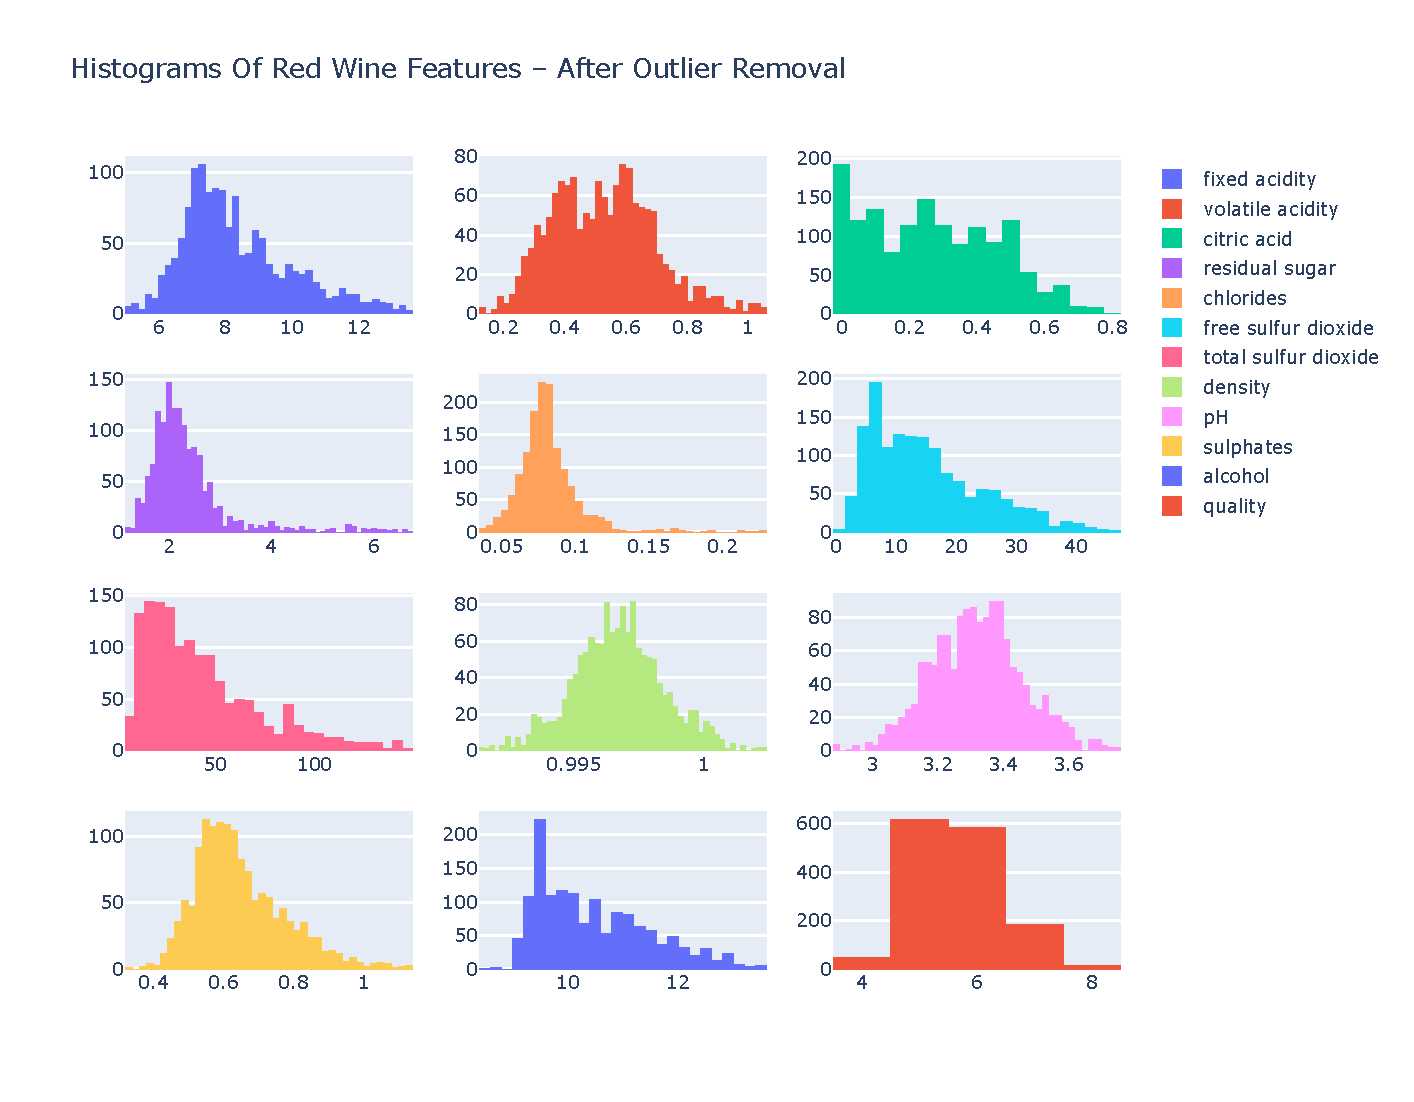
\includegraphics[width=0.75\textwidth]{figures/redwinehisto2}
    \caption{Red wine features histograms after outlier removal.}%
    \label{fig:redwinehisto2}
  \end{figure} 

  \subsection{Principal component analysis}

  PCA is performed in Listing~\ref{lst:pcaredwine} to visualize correlations
  between the different features in the \lstinline{winequality-red} dataset.
  All features are scaled to zero mean and unit variance beforehand (otherwise
  PCA might determine that the direction of maximal variance corresponds to
  features varying more than others because of their scales).

  Figure~\ref{fig:pcaredwine} shows two plots used to study correlations:
  \begin{itemize}
    \item a scree plot, showing eigenvalues ordered from largest to smallest.
      This plot can be used to determine the number of eigenvalues to keep for
      a later analysis;
    \item a variables factor map, showing the correlations between all twelve
      features and the top two principal components. Features that are grouped
      together are positively correlated, while features on opposite sides of
      the unit circle are negatively correlated.
  \end{itemize}

  \begin{lstlisting}[caption={PCA and correlation plots.}, captionpos=b,
    label={lst:pcaredwine}]
# Cleaned dataset is scaled to zero mean and unit variance.
red_wine_norm = pd.DataFrame(
  StandardScaler().fit_transform(red_wine_clean),
  columns=red_wine_clean.columns
)

# Fit PCA model.
pca_model = PCA()
pca_result = pca_model.fit_transform(red_wine_norm)

# Get correlations between components and features.
coef = pd.DataFrame(pca_model.components_.T[:, 0:2],
                    columns=["pc1", "pc2"],
                    index = red_wine.columns)

fig = make_subplots(rows=1, cols=2,
                    subplot_titles=("Scree Plot", "Variables Factor Map"))

# Scree plot.
fig.add_trace(
  go.Bar(
    x=["PC {}".format(i) for i in range(1, pca_model.components_.shape[1]+1)],
    y=pca_model.explained_variance_ratio_,
    name="Scree Plot"
  ),
  row=1,
  col=1
)

# Variables factor map.
# The angle in the unit circle is used to compute the point color. This way
# correlated features will appear with similar colors.
fig.add_trace(
  go.Scatter(
    x=coef.pc1,
    y=coef.pc2,
    text=red_wine.columns,
    mode="markers+text",
    textposition="top center",
    marker=dict(
      size=10,
      color=np.angle(coef.pc1 + 1j*coef.pc2, deg=True)
    ),
    name="Variables Factor Map"
  ),
  row=1,
  col=2
)

# Add unit circle.
fig.update_layout(
  shapes=[
    # unfilled circle
    dict(
      type="circle",
      xref="x2",
      yref="y2",
      x0=-1,
      y0=-1,
      x1=1,
      y1=1
    ),
  ]
)
    
# Update figure size, axes titles and remove legend.
fig.update_layout(
  height=600, 
  width=1200, 
  showlegend=False,
  xaxis_title="Component Number",
  yaxis_title="Explained Variance Ratio",
  xaxis2_title="PCA 1 ({:.2f}%)".format(pca_model.explained_variance_ratio_[0]*100),
  yaxis2_title="PCA 2 ({:.2f}%)".format(pca_model.explained_variance_ratio_[1]*100)
)

fig.show(width=1400)
  \end{lstlisting}

  \begin{figure}[!ht]
    \centering
    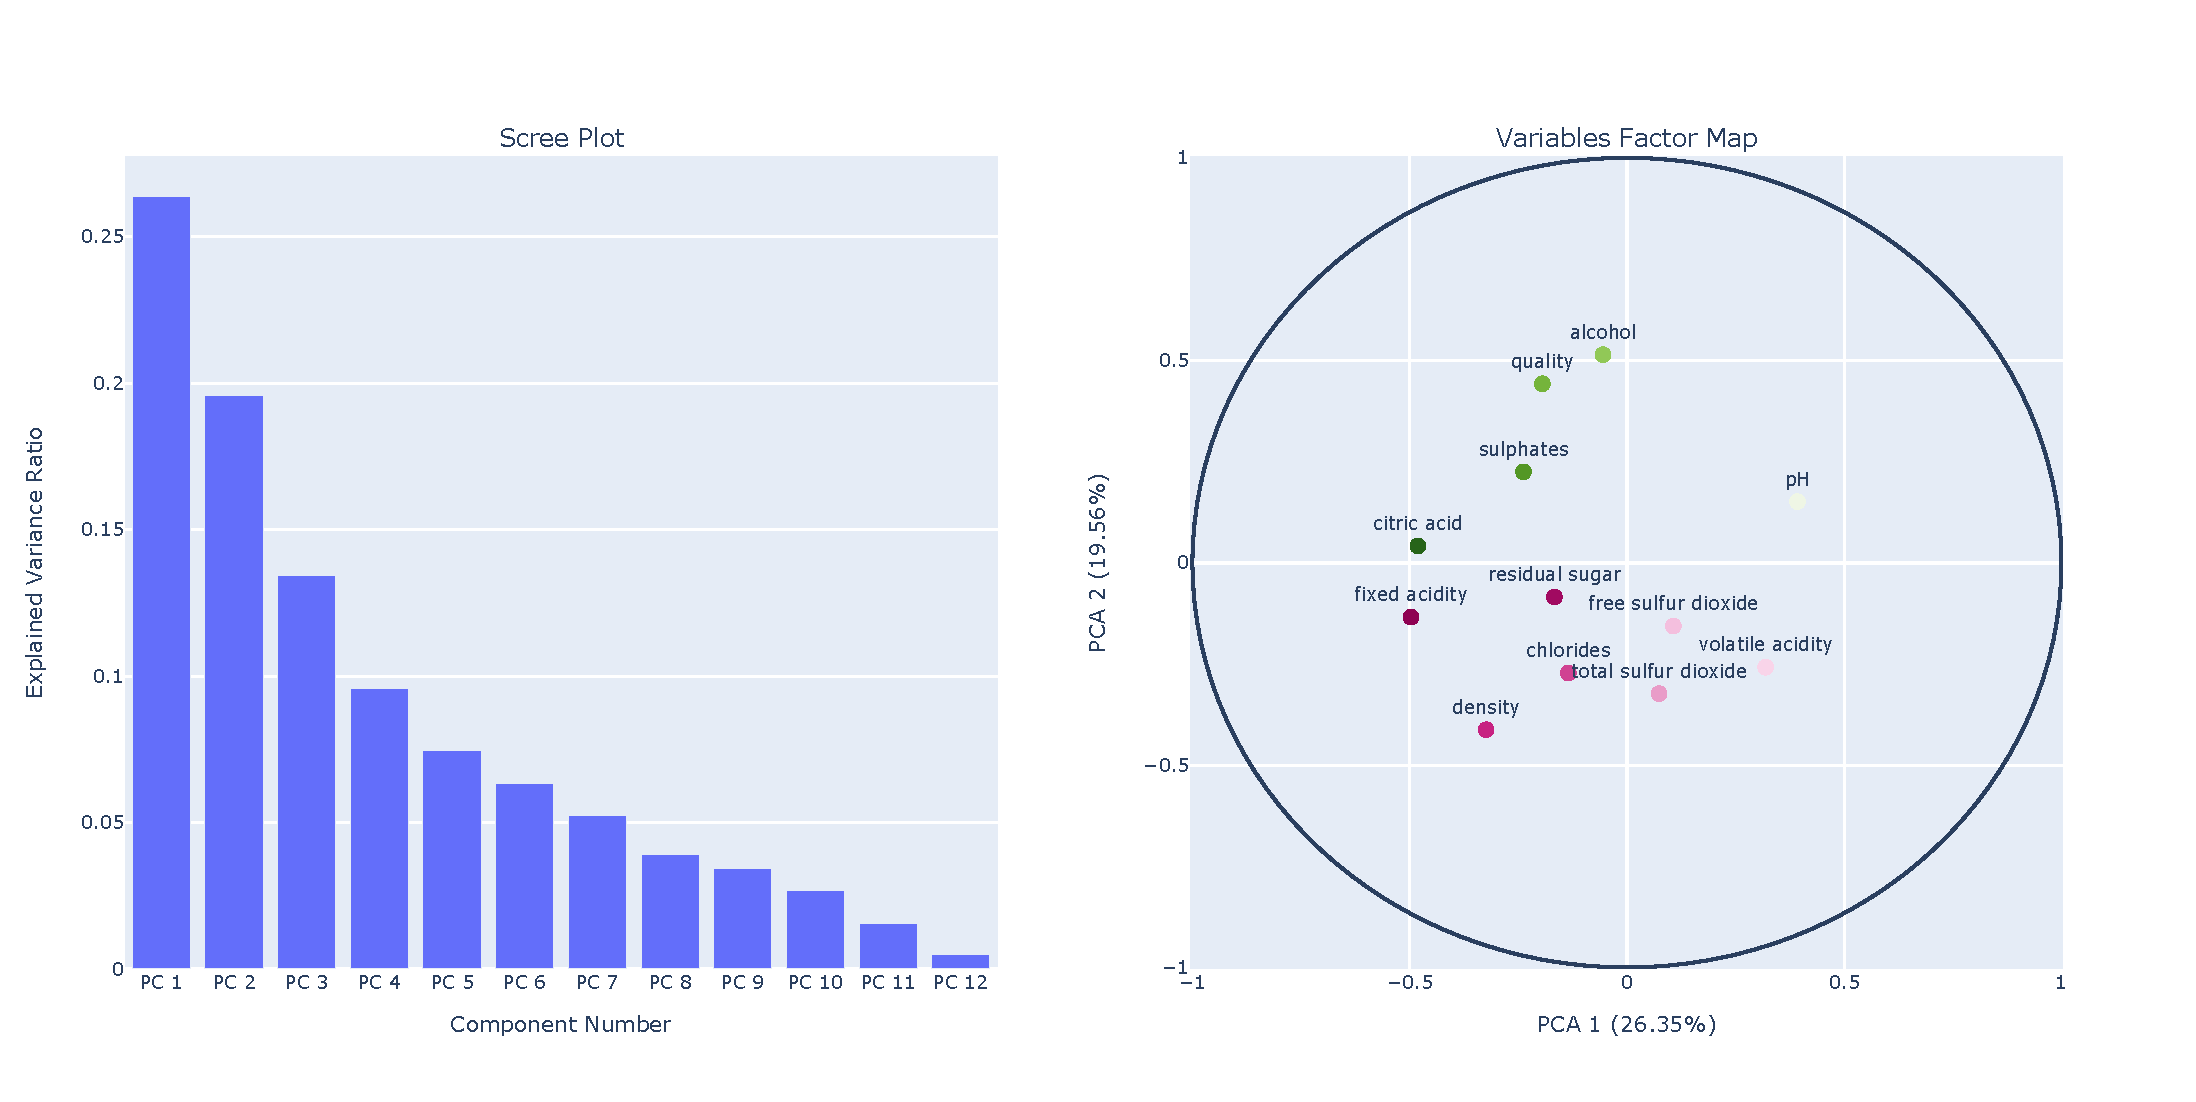
\includegraphics[width=\textwidth]{figures/pcaredwine}
    \caption{Scree plot and variables factor map from the principal component
      analysis of red wine features.}%
    \label{fig:pcaredwine}
  \end{figure} 

  The scree plot shows that the top two principal components explain about 45\%
  of the variance in the data. Therefore, using only the top two components to
  analyse the data is risky, as a lot of information is lost in the higher
  dimensions.

  On the variables factor map, using the top two components, we observe: 
  \begin{itemize}
    \item a strong positive correlation between the alcohol and quality
      features, with a slightly weaker correlation between these features and
      the sulphates.
    \item a strong negative correlation between the alcohol, quality and
    sulphates features and the volatile acidity, total sulfur dioxide and free
    sulfur dioxide features.
  \end{itemize}

  As previously stated, considering that the rest of the components still
  explain a significant part of the variance, the variables factor map should
  be interpreted with caution: in higher dimensions, some of these points could
  be farther apart than seen on a 2D visualization.

  \subsection{Multivariate linear regression}

  In Listing~\ref{lst:mlr}, we perform multivariate linear regression (ordinary
  least squares) of the \lstinline{quality} score against the remaining 11
  input features (with intercept).

  \begin{lstlisting}[caption={Multivariate linear regression of the quality
    score against all input features.}, captionpos=b, label={lst:mlr}]
# Standardize input features (zero mean, with or without unit variance).
X_mean_removed = StandardScaler(with_std=False).fit_transform(red_wine_clean.drop("quality", axis=1))
X_norm = StandardScaler().fit_transform(red_wine_clean.drop("quality", axis=1))

y = red_wine_clean.quality

# Perform multivariate linear regression.
est_zero_mean = sm.OLS(y, sm.add_constant(X_mean_removed)).fit()
est_norm = sm.OLS(y, sm.add_constant(X_norm)).fit()

# Plot regression coefficients as grouped bar plots.
# Significant coefficients are colored in red, non-significant in gray.
fig = make_subplots(
  rows=2, cols=1, 
  shared_xaxes=True, 
  vertical_spacing=0.1,
  subplot_titles=("Zero Mean", "Zero Mean, Unit Variance")
)

fig.add_trace(
  go.Bar(
    x=red_wine.columns,
    y=est_zero_mean.params[1:],
    name="Zero Mean",
    marker_color=["crimson" if p <= 0.05 else "lightslategray" for p in est_zero_mean.pvalues[1:]]
  ),
  row=1,
  col=1
)
fig.add_trace(
  go.Bar(
    x=red_wine.columns,
    y=est_norm.params[1:],
    name="Zero Mean, Unit Variance",
    marker_color=["crimson" if p <= 0.05 else "lightslategray" for p in est_norm.pvalues[1:]]
  ),
  row=2,
  col=1
)

fig.update_layout(
  title="Multivariate Linear Regression Coefficients, R^2 = {:.2f}, red: p < 0.05 ".format(est_norm.rsquared),
  showlegend=False,
  height=800
)
fig.show()
  \end{lstlisting}

  Figure~\ref{fig:mlr} shows a comparison of the estimated model parameters
  when the input features have been standardized either by simply scaling to
  zero mean, or by by both scaling to zero mean and unit variance.

  \begin{figure}[!ht]
    \centering
    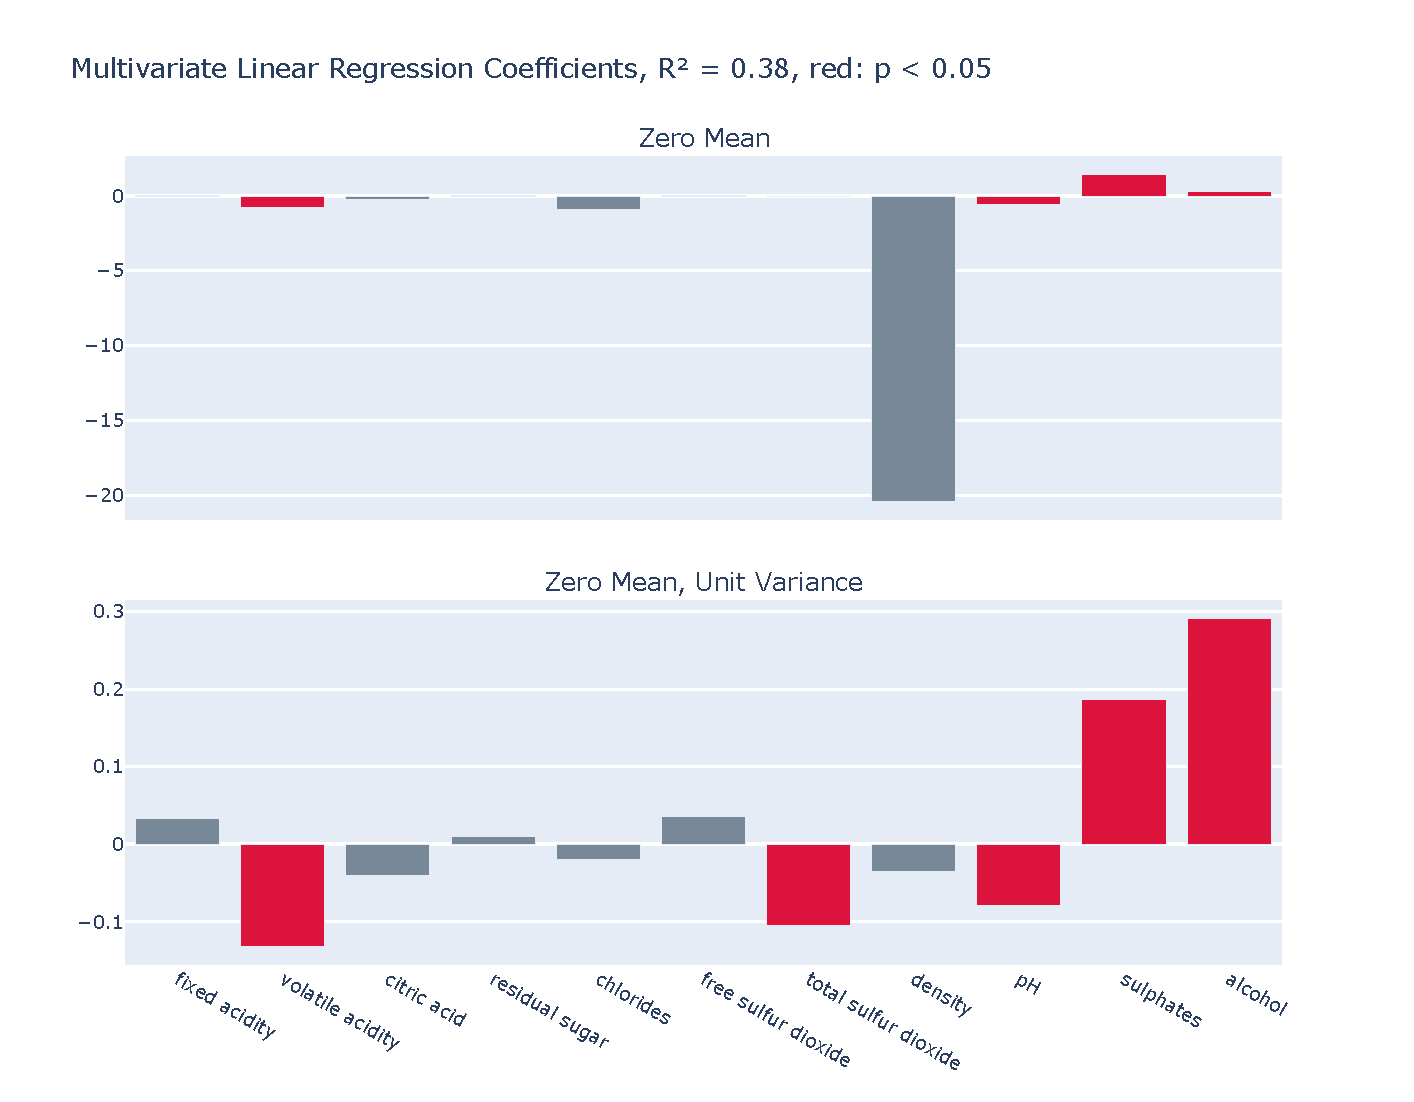
\includegraphics[width=\textwidth]{figures/mlr}
    \caption{Bar plots comparing the estimated model parameters in two
    conditions. Significant parameters at the 5\% confidence level are colored
    in red. (\textbf{Top}) input features have been standardized by scaling
    to zero mean. (\textbf{Down}) input features have been standardized by
    scaling to zero mean and unit variance.}%
    \label{fig:mlr}
  \end{figure} 

  The intercept term isn't displayed as it would hinder the visualization (it
  correponds to the mean of the \lstinline{quality} score). As expected, the
  standard scaling of the dataset prior to regression (zero mean and unit
  variance) is essential to interpret the results: when the individual features
  aren't comparable due to their difference in scales, their respective
  regression coefficients aren't comparable either.

  The coefficient of determination doesn't change between both settings, as it
  is already normalized (normalized covariance). Its value is relatively low:
  the current model including all input features and an intercept term explains
  only about 38\% of the variance of the \lstinline{quality} feature. Looking
  back at the histogram of the \lstinline{quality} feature, we can see that it
  has very low variance, with most scores being either 5 or 6. Seeing that the
  difference in \lstinline{quality} between the wines is almost binary, the
  multivariate linear model isn't well suited. To obtain better predictions,
  further processing of the \lstinline{quality} feature would be necessary
  (e.g.\ using a continuous scale), or a new model could be used (e.g.\
  multivariate logistic regression, by binarizing the \lstinline{quality}
  score).

  Most regression coefficients aren't significant at the 5\% level: the
  significant features are colored in red on the above box plots. From the
  remaining features, we observe that
  \begin{itemize}
    \item the \lstinline{alcohol} and \lstinline{sulphates} features show
      positive influence on the \lstinline{quality} score;
    \item the \lstinline{volatile acidity}, \lstinline{total sulfur dioxide}
      and \lstinline{pH} features show negative influence on the
      \lstinline{quality} score.
  \end{itemize}

  \subsection{Lasso regression and model selection}

  As the OLS model including all input features was inaccurate, lasso is
  suggested in this section as a way to select relevant features for the
  prediction of \lstinline{quality}. However, lasso is likely to suffer the
  same fate as OLS, as it won't be able to explain more variance than the full
  OLS model.

  In Listing~\ref{lst:lasso}, the lasso model is fitted along a given
  regularization path: $\alpha\in[10^{-3}, 1]$. To assess performance, the
  cleaned dataset is split into a training set of size 500 and a testing
  test of size 941. A scaler for zero mean and unit variance is fitted on the
  training set and the transformation applied on both training and testing
  sets. Finally, to find the best model, 10-fold cross-validation is used along
  the regularization path.

  \begin{lstlisting}[caption={Lasso regression of the quality score against all
    input features, along a given regularization path.}, captionpos=b,
    label={lst:lasso}]
# Split dataset into testing and training set.
X_train, X_test, y_train, y_test = train_test_split(
  red_wine_clean.drop("quality", axis=1), 
  red_wine_clean.quality, 
  train_size=500, 
  random_state=42
)

# Standardize data, fitting only on training set.
sc = StandardScaler()
X_train = sc.fit_transform(X_train)
X_test = sc.transform(X_test)

_, n = X_train.shape

# Regularization parameters path.
alphas = np.logspace(-3, 0, 100)

# Compute lasso path with coordinate descent.
alphas_lasso, coefs_lasso, _ = lasso_path(X_train, y_train, alphas=alphas, random_state=42)

# Compute lasso with iterative fitting along the regularization path.
# The best model is chosen by 10-fold cross-validation.
model = LassoCV(cv=10, alphas=alphas, random_state=42).fit(X_train, y_train)

# Compute training and testing score (R^2) along the regularization path.
training_score = []
testing_score = []
for a in alphas:
  reg = Lasso(alpha=a, random_state=42).fit(X_train, y_train)
  training_score.append(reg.score(X_train, y_train))
  testing_score.append(reg.score(X_test, y_test))

# Plot lasso coefficients, MSE and performance along the regularization path.
fig = make_subplots(
  rows=3, 
  cols=1, 
  vertical_spacing=0.1,
  subplot_titles=("Lasso Path", "K-Fold Cross-Validation, K = 10", "Lasso Performance")
)

# Lasso coefficients.
for i in range(n):
  fig.add_trace(
    go.Scatter(
      x=alphas_lasso,
      y=coefs_lasso[i],
      name=red_wine_clean.columns[i],
      mode="lines",
      legendgroup="lasso"
    ),
    row=1,
    col=1
  )

# Lasso MSE.
for i in range(10):
  fig.add_trace(
    go.Scatter(
      x=model.alphas_,
      y=model.mse_path_[:, i],
      mode="lines",
      line=dict(dash="dot"),
      marker_color="grey",
      showlegend=False,
      name="MSE {}".format(i)
    ),
    row=2,
    col=1
  )
fig.add_trace(
  go.Scatter(
    x=model.alphas_,
    y=model.mse_path_.mean(axis=1),
    mode="lines",
    marker_color="black",
    legendgroup="cv",
    name="Average MSE"
  ),
  row=2,
  col=1
)

# Lasso performance.
fig.add_trace(
  go.Scatter(
    x=alphas,
    y=training_score,
    mode="lines",
    legendgroup="performance",
    name="Training"
  ),
  row=3,
  col=1
)
fig.add_trace(
  go.Scatter(
    x=alphas,
    y=testing_score,
    mode="lines",
    legendgroup="performance",
    name="Testing"
  ),
  row=3,
  col=1
)

# Add dashed line on each plot to indicate the regularization factor for the best model.
min_alpha = model.alphas_[np.argmin(model.mse_path_.mean(axis=1))]
fig.add_shape(
  go.layout.Shape(
    type="line",
    yref="y",
    xref="x",
    x0=min_alpha,
    y0=-0.2,
    x1=min_alpha,
    y1=0.43,
    line=dict(dash="dot")
  ),
  row=1,
  col=1
)
fig.add_shape(
  go.layout.Shape(
    type="line",
    yref="y",
    xref="x",
    x0=min_alpha,
    y0=-0.2,
    x1=min_alpha,
    y1=0.43,
    line=dict(dash="dot")
  ),
  row=1,
  col=1
)
fig.add_shape(
  go.layout.Shape(
    type="line",
    yref="y",
    xref="x",
    x0=min_alpha,
    y0=0.27,
    x1=min_alpha,
    y1=0.9,
    line=dict(dash="dot")
  ),
  row=2,
  col=1
)
fig.add_shape(
  go.layout.Shape(
    type="line",
    yref="y",
    xref="x",
    x0=min_alpha,
    y0=-0.05,
    x1=min_alpha,
    y1=0.4,
    line=dict(dash="dot")
  ),
  row=3,
  col=1
)

fig.update_layout(
  xaxis_type="log", 
  xaxis2_type="log",
  xaxis3_type="log",
  xaxis3_title="Regularization Parameter",
  yaxis_title="Lasso coefficients",
  yaxis2_title="Validation Sets MSE",
  yaxis3_title="Model Performance (R^2)",
  height=800
)
    
fig.show()
  \end{lstlisting}

  \begin{figure}[!ht]
    \centering
    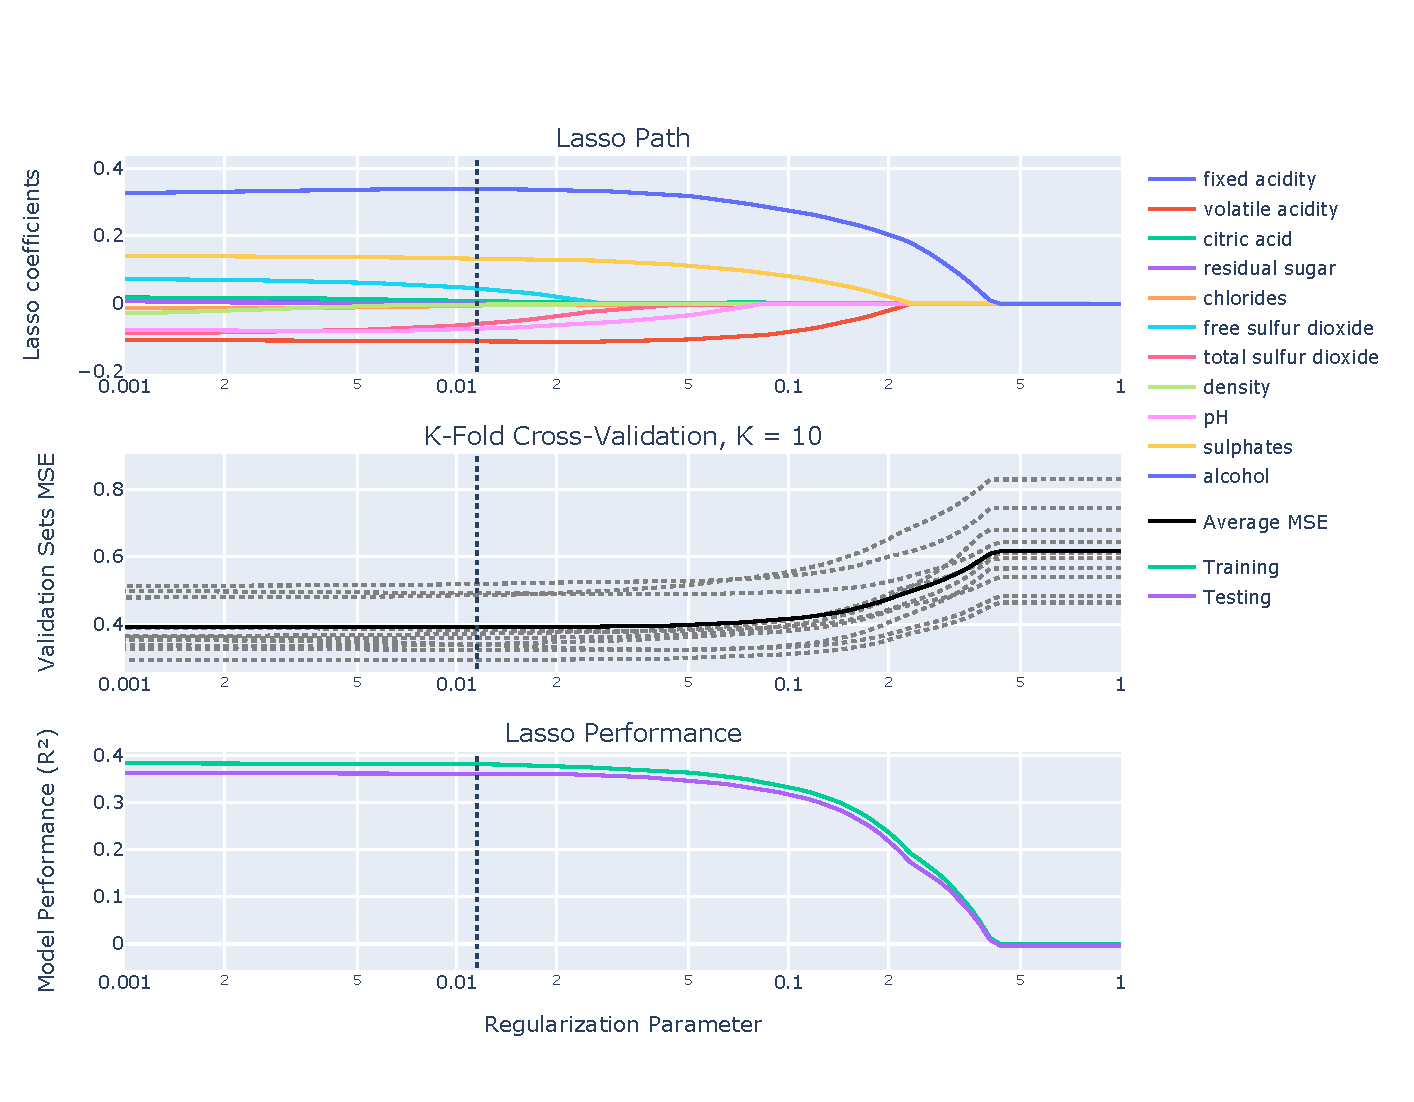
\includegraphics[width=\textwidth]{figures/lasso}
    \caption{Lasso regression of the quality score against all input features,
    along a given regularization path. (\textbf{Top}) Evolution of the lasso
    coefficients with the regularization parameter. (\textbf{Middle}) Evolution
    of the mean squared error of each validation set from a 10-fold
    cross-validation. (\textbf{Bottom}) Evolution of lasso performance with the
    regularization parameter.}%
    \label{fig:lasso}
  \end{figure} 

  The dashed line across all plots of Figure~\ref{fig:lasso} represents the
  best model obtained through 10-fold cross-validation. For this optimal model,
  the lasso regression mainly includes:
  \begin{itemize}
    \item the \lstinline{alcohol} and \lstinline{sulphates} features,
      contributing positively to the \lstinline{quality}; 
    \item the \lstinline{volatile acidity} feature contributing negatively to
      the \lstinline{quality}.
  \end{itemize}

  This result is very close to the significant features found in the OLS model.
  Unexpectedly, the performance of the optimal lasso model is similar to the
  performance of the previous OLS model. Moreover, the benefit of
  cross-validation on this task seems negligible, considering the flatness of
  the average MSE\@. We can once again conclude that a linear model isn't well
  suited to this task.

  \subsection{Next steps}

  Since the previous linear models were not able to accurately predict the
  \lstinline{quality} of red wines, we are interested in knowing if a new model
  that takes into account the previous observations could do better. Since the
  \lstinline{quality} is almost binary, as seen on the first histogram, we fix
  an arbitrary threshold in Listing~\ref{lst:qualitybinary} that will
  discriminate between \textit{good} and \textit{bad} wines.  This threshold is
  fixed at a \lstinline{quality} of 5.5, so that wines with a score of 5 or
  lower will be rated as \textit{bad}. Figure~\ref{fig:qualitybinary} shows the
  counts for each quality.

  \begin{lstlisting}[caption={Binarize the quality feature.}, captionpos=b,
    label={lst:qualitybinary}]
# Deep copy used so that the original dataset isn't modified.
red_wine_bin = red_wine_clean.copy(deep=True)

# Binarize the quality feature into "good" and "bad" wines.
bins = (2, 5.5, 8)
group_names = ["bad", "good"]
red_wine_bin["quality"] = pd.cut(red_wine_bin.quality, bins=bins, labels=group_names)

# Bar plot of wine quality.
fig = go.Figure(go.Bar(
  x=["bad", "good"],
  y=red_wine_bin.quality.value_counts()
))

fig.update_layout(
  title="Red Wine Quality - Binarized",
  xaxis_title="Quality",
  yaxis_title="Count",
  height=800
)

fig.show(height=300)
  \end{lstlisting}

  \begin{figure}[!ht]
    \centering
    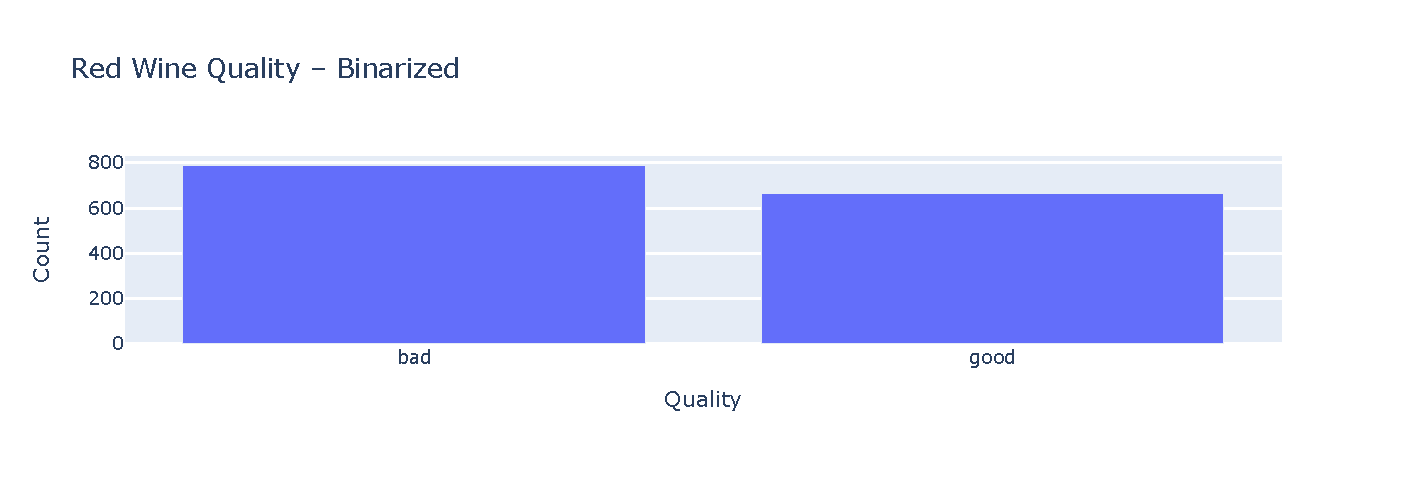
\includegraphics[width=\textwidth]{figures/qualitybinary}
    \caption{Red wine binarized quality counts.}%
    \label{fig:qualitybinary}
  \end{figure} 

  In Listing~\ref{lst:qualitysvm}, the dataset is split into training and
  testing sets, with a more common 80\%/20\% ratio. The input features are
  standardized to get optimal results. A linear SVM model is used for
  classification, because of its ease of use.
  
  \newpage

  \begin{lstlisting}[caption={Linear SVM classifier of red wine quality.},
    captionpos=b, label={lst:qualitysvm}]
# Split dataset into training and testing sets.
X_train, X_test, y_train, y_test = train_test_split(
  red_wine_bin.drop("quality", axis=1), 
  red_wine_bin.quality, 
  test_size=0.2, 
  random_state=42
)

# Standardize input features.
sc = StandardScaler()
X_train = sc.fit_transform(X_train)
X_test = sc.transform(X_test)

clf = LinearSVC(max_iter=2000)
clf.fit(X_train, y_train)

print("Classification report on the testing test:\n")
print(classification_report(y_test, clf.predict(X_test)))

#Classification report on the testing test:
#
#              precision    recall  f1-score   support
#
#         bad       0.69      0.69      0.69       131
#        good       0.74      0.74      0.74       160
#
#    accuracy                           0.72       291
#   macro avg       0.72      0.72      0.72       291
#weighted avg       0.72      0.72      0.72       291
  \end{lstlisting}

  We obtain a mean precision and recall on the testing set of about 72\%. This
  performance could be slightly improved by using cross-validation and a
  non-linear SVM (kernel trick), but other methods (random forest, k-NN, etc.)
  should probably show better performances.

  \subsection{Classification}

  In this section, we will try to classify wine color from their
  physicochemical properties, using datasets \lstinline{winequality-red} and
  \lstinline{winequality-white}. In Listing~\ref{lst:whiteclean}, the white
  wine dataset is cleaned out of outliers using the same criterion as before
  (outliers outside the $\pm 3$ standard deviations range are removed) and
  merged with the clean red wine dataset. A \lstinline{color} feature is added
  to the dataset to distinguish red from white wines. The \lstinline{quality}
  feature is removed as it won't be used by the classifier.
  Figure~\ref{fig:whiteclean} shows the features histograms for the merged
  datasets.

  \begin{lstlisting}[caption={Clean and merge white wine dataset.},
    captionpos=b, label={lst:whiteclean}]
# Read white wine dataset and apply the same cleaning procedure as before.
white_wine = pd.read_csv("data/winequality/winequality-white.csv", sep=";")
white_wine_clean = white_wine[(np.abs(stats.zscore(white_wine)) < 3).all(axis=1)]

# Add color feature and merge datasets.
wine = pd.concat([red_wine_clean.assign(color="red"), white_wine_clean.assign(color="white")]).drop("quality", axis=1)

# Plot histograms for each variable.
fig = make_subplots(rows=4, cols=3)

for i, col in enumerate(wine.columns, 1):
  fig.add_trace(
    go.Histogram(
      x=wine[col],
      name=col
    ), 
    row=int(np.ceil(i / 3)), 
    col=i % 3 if i % 3 != 0 else 3
  )
    
fig.update_layout(
  title_text="Histograms Of Red and White Wine Features",
  height=800
)

fig.show()
  \end{lstlisting}

  \begin{figure}[!ht]
    \centering
    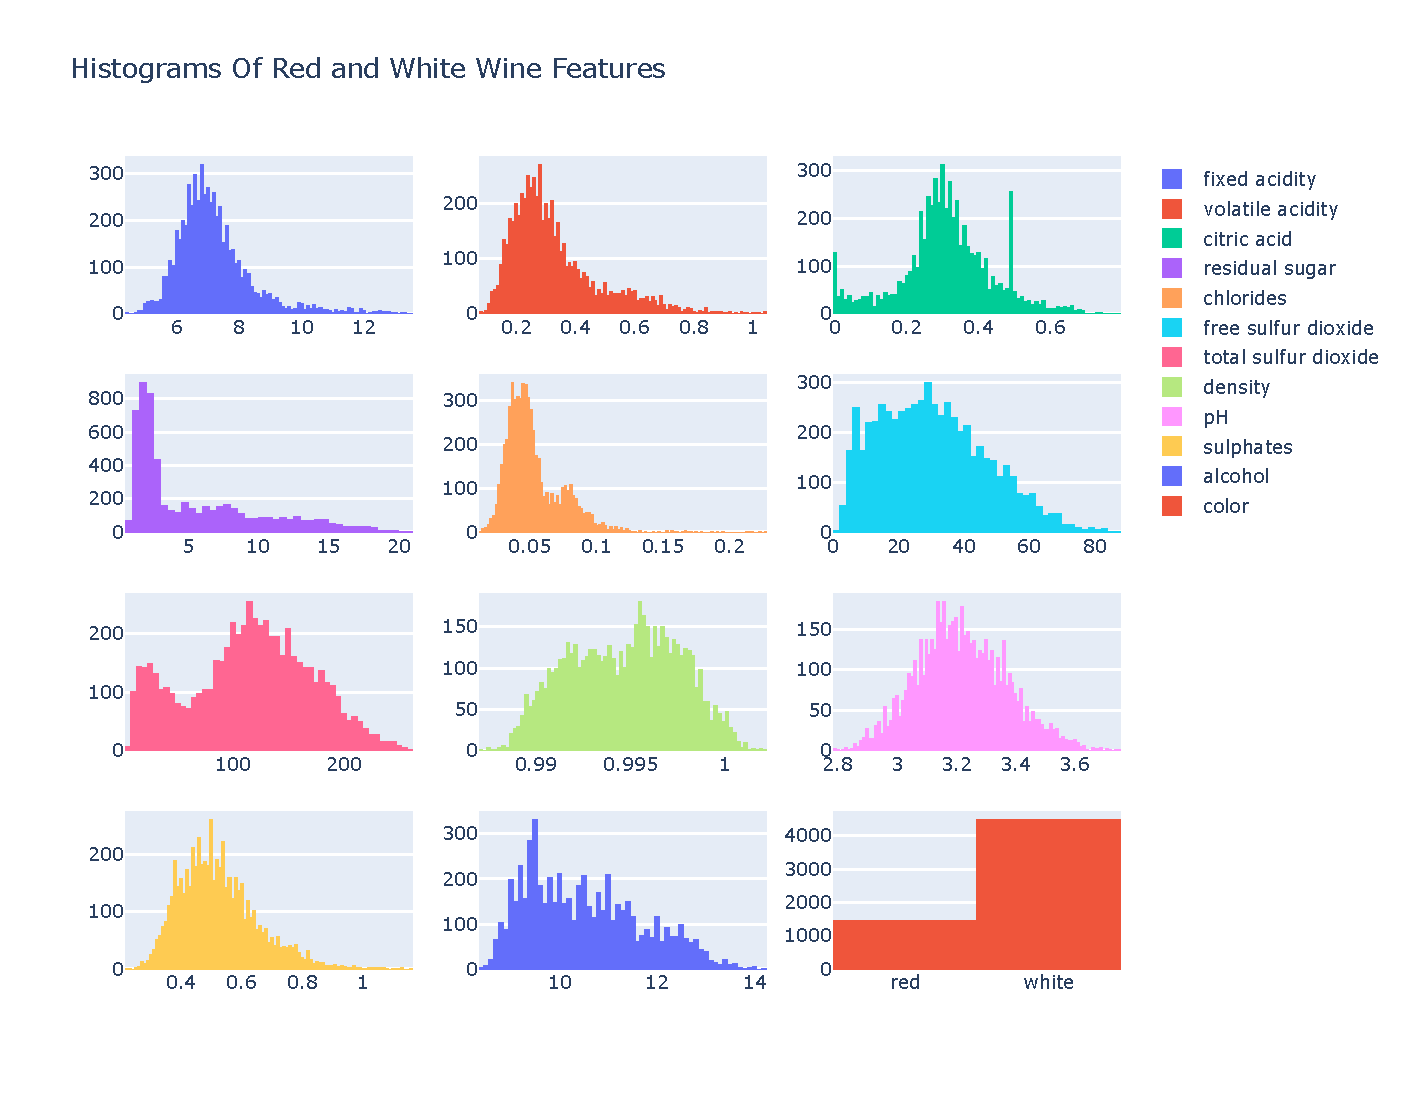
\includegraphics[width=0.75\textwidth]{figures/wineshisto}
    \caption{Red and white wines features histograms after outlier removal.}%
    \label{fig:whiteclean}
  \end{figure} 

  \newpage

  With both datasets merged, we observe that some histograms are bimodal, which
  could indicate that these features will enable discrimination of red and
  white wines. Figure~\ref{fig:scatterwines} shows a scatter plot of
  \lstinline{chlorides} vs. \lstinline{total sulfur dioxide}, two features that
  shows bimodal histograms, obtained using Listing~\ref{lst:scatterwines}.

  \begin{lstlisting}[caption={Scatter plot of chlorides vs.\ total sulfur
    dioxide.}, captionpos=b, label={lst:scatterwines}]
# Scatter plot chlorides vs. total sulfur dioxide.
fig = go.Figure()

fig.add_trace(go.Scatter(
  x=wine.loc[wine.color == "white", "total sulfur dioxide"],
  y=wine.loc[wine.color == "white", "chlorides"],
  mode="markers",
  name="White Wines"
))
fig.add_trace(go.Scatter(
  x=wine.loc[wine.color == "red", "total sulfur dioxide"],
  y=wine.loc[wine.color == "red", "chlorides"],
  mode="markers",
  name="Red Wines"
))

fig.update_layout(
  title="Chlorides vs. Total Sulfur Dioxide",
  xaxis_title="Total Sulfur Dioxide",
  yaxis_title="Chlorides",
  height=800
)

fig.show()
  \end{lstlisting}

  \begin{figure}[!ht]
    \centering
    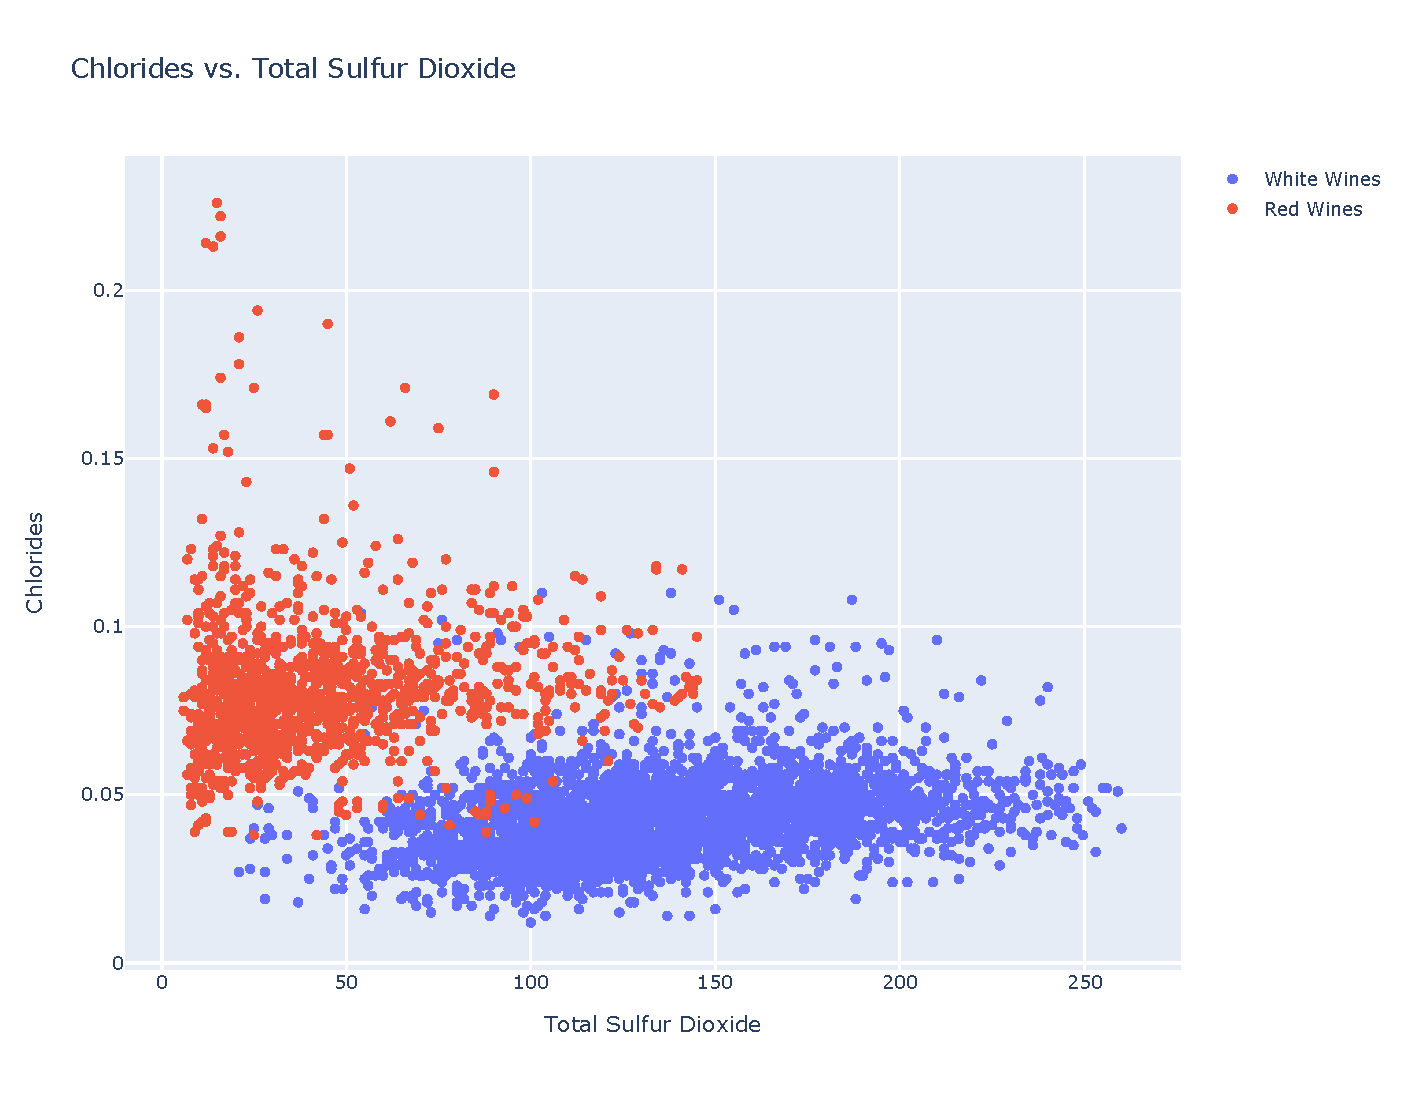
\includegraphics[width=\textwidth]{figures/scatterwines}
    \caption{Scatter plot of chlorides vs.\ total sulfur dioxide.}%
    \label{fig:scatterwines}
  \end{figure} 

  Indeed, using only two features, wines can be almost perfectly visually
  classified according to their color. Given its ease of use compared to a PCA
  + $k$-mean clustering classifier, a linear SVM model is used once again in
  Listing~\ref{lst:winesvm}.  Considering the observations on the histograms,
  the dataset is split into training and testing sets using a 10\%/90\% ratio.

  \begin{lstlisting}[caption={Linear SVM classifier of wine color.},
    captionpos=b, label={lst:winesvm}]
# Split dataset into training and testing sets.
X_train, X_test, y_train, y_test = train_test_split(
  wine.drop("color", axis=1), 
  wine.color, 
  test_size=0.90, 
  random_state=42
)

# Standardize input features.
sc = StandardScaler()
sc.fit(X_train)
X_train = sc.transform(X_train)
X_test = sc.transform(X_test)

# Fit linear SVM and print accuracy.
clf = LinearSVC(max_iter=2000)
clf.fit(X_train, y_train)

print("Mean accuracy on training set: {:.2f}%".format(100*clf.score(X_train, y_train)))
print("Mean accuracy on testing set: {:.2f}%".format(100*clf.score(X_test, y_test)))

#Mean accuracy on training set: 100.00%
#Mean accuracy on testing set: 99.76%
  \end{lstlisting}

  The linear SVM classifier is perfectly suited for this task: the error on the
  testing set is only about 0.2\%. Finally, we can study which variables should
  be kept to keep this error below 1\%. The \lstinline{chlorides},
  \lstinline{total sulfur dioxide}, \lstinline{density} and
  \lstinline{residual sugar} features are selected based on their histograms
  and a new linear SVM classifier is fitted using this reduced dataset in
  Listing~\ref{lst:winesvm2}.

  \begin{lstlisting}[caption={Linear SVM classifier of wine color.},
    captionpos=b, label={lst:winesvm2}]
# Split dataset into training and testing sets.
wine_test = wine[["chlorides", "total sulfur dioxide", "density", "residual sugar", "color"]]

X_train, X_test, y_train, y_test = train_test_split(
    wine_test.drop("color", axis=1), 
    wine_test.color, 
    test_size=0.90, 
    random_state=42
)

# Standardize input features.
sc = StandardScaler()
sc.fit(X_train)
X_train = sc.transform(X_train)
X_test = sc.transform(X_test)

# Fit linear SVM and print accuracy.
clf = LinearSVC(max_iter=2000)
clf.fit(X_train, y_train)

print("Mean accuracy on training set: {:.2f}%".format(100*clf.score(X_train, y_train)))
print("Mean accuracy on testing set: {:.2f}%".format(100*clf.score(X_test, y_test)))

#Mean accuracy on training set: 99.33%
#Mean accuracy on testing set: 99.33%
  \end{lstlisting}

  As we can see, keeping only these features, the test error is only about
  0.7\%: we were able to reduce the dataset to only four input features.
  Therefore, measuring only these four physicochemical properties should be
  sufficient to achieve a good color classification.

  \section{Clustering of handwritten digits}

  In this section, we consider the Handwritten Digits Data Set (E. Alpaydin
  \textit{et al.}, 1998), available on the
  \href{https://archive.ics.uci.edu/ml/machine-learning-databases/optdigits/}{UC
  Irvine Machine Learning Repository}, and in particular the
  \lstinline{optdigits.tes} testing dataset.

  The dataset was obtained by processing $32 \times 32$ normalized bitmaps of
  handwritten digits. These bitmaps were divided into nonoverlapping $4 \times
  4$ blocks and the number of \textit{on} pixels were counted in each block.
  This operation reduced each bitmap to an $8 \times 8$ input matrix where each
  element is an integer in the range $[0, 16]$. Each row of the
  \lstinline{optidigits.tes} dataset contains an $8 \times 8$ matrix reshaped
  to a horizontal $1 \times 64$ vector, with an additional class attribute
  column specifying the digit.

  The goal of this section is to cluster the data without taking into account
  the labels, thus studying an unsupervised learning method. The class
  attribute column containing the label will be used to assess the results.

  In Listing~\ref{lst:readdigits}, the data is read and the 64 input features
  are standardized to zero mean and unit variance. Figure~\ref{lst:readdigits}
  shows some digits examples from the dataset. As we can see, even with the
  dimension reduction applied by the authors, most digits are still
  identifiable.

  \begin{lstlisting}[caption={Read handwritten digits dataset and display
    example images.}, captionpos=b, label={lst:readdigits}]
# Read dataset and separate input features and labels.
dig = np.loadtxt("data/optdigits.tes", dtype='i', delimiter=',')
X = dig[:, :-1]
y = dig[:, -1]

n, m = X.shape

# Plot some examples from the dataset.
fig = make_subplots(rows=3, cols=3)

for i in range(1,10):
  fig.add_trace(
    go.Heatmap(
      z=np.flip(X[i, :].reshape((8, 8)), 0),
      showscale=False,
      colorscale="gray",
      name="Label: {}".format(y[i])
    ),
    row=int(np.ceil(i / 3)),
    col=i % 3 if i % 3 != 0 else 3
  )

fig.update_layout(
  title="Handwritten Digits Dataset, Examples",
  height=800,
  width=800
)

fig.show(height=900)

# Standardize input features.
X_norm = StandardScaler().fit_transform(X)
  \end{lstlisting}

  \begin{figure}[!ht]
    \centering
    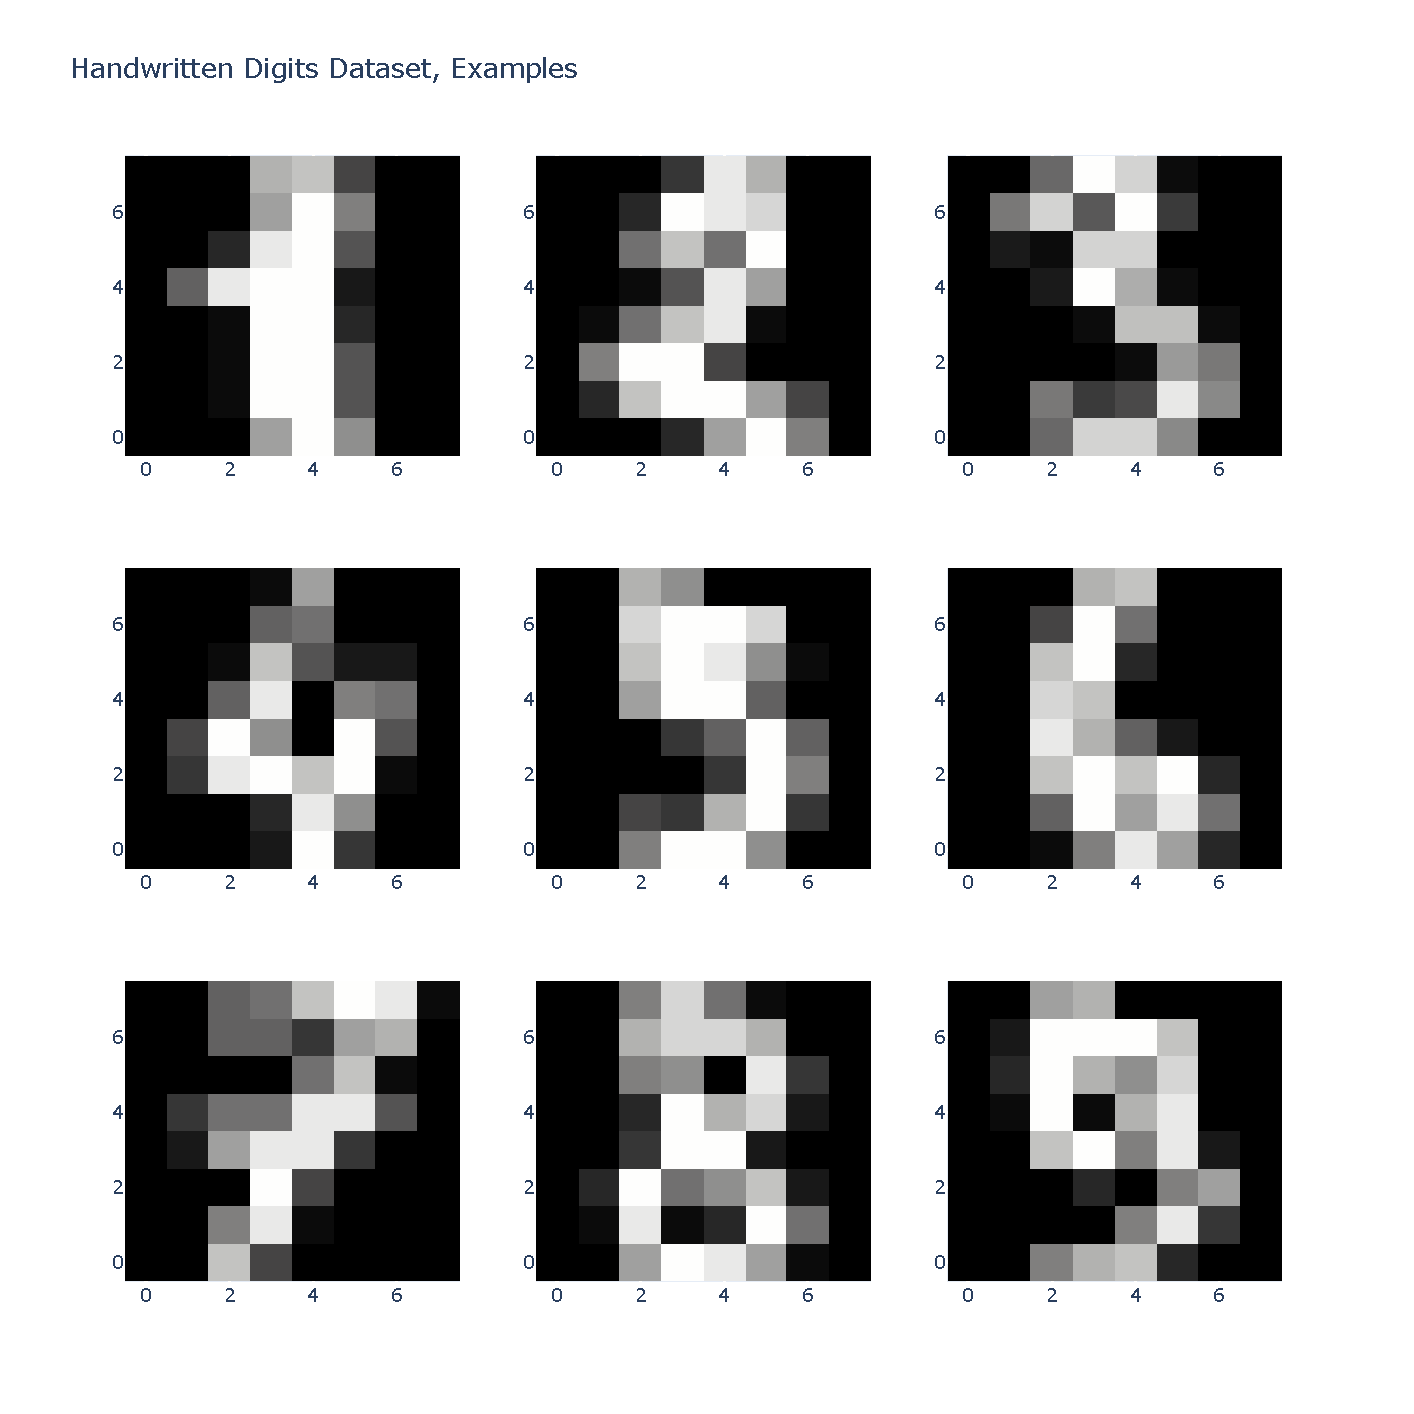
\includegraphics[width=0.7\textwidth]{figures/readdigits}
    \caption{Handwritten digits examples}%
    \label{fig:readdigits}
  \end{figure} 

  \subsection{$K$-means clustering}

  In this section, a $K$-means clustering method will be applied to cluster the
  data. First, we would like to find a good 2D visualization of the dataset.
  Figure~\ref{fig:digitspca} shows the projection of the data on the top two
  principal components obtained from a PCA performed in
  Listing~\ref{lst:digitspca}.

  \begin{lstlisting}[caption={Perform PCA and project on top two components.},
    captionpos=b, label={lst:digitspca}]
# Perform PCA and plot the projected input features on top 2 components.
pca_model = PCA()
pca_result = pca_model.fit_transform(X_norm)

fig = go.Figure()

for i in range(10):
  fig.add_trace(go.Scatter(
    x=pca_result[y==i, 0],
    y=pca_result[y==i, 1],
    mode="markers",
    marker_color=i,
    name="True Label: {}".format(i)
  ))
    
fig.update_layout(
  title="PCA Visualization Of Handwritten Digits",
  xaxis_title="PCA 1 ({:.2f}%)".format(pca_model.explained_variance_ratio_[0]*100),
  yaxis_title="PCA 2 ({:.2f}%)".format(pca_model.explained_variance_ratio_[1]*100),
  height=800
)

fig.show()
  \end{lstlisting}

  \begin{figure}[!ht]
    \centering
    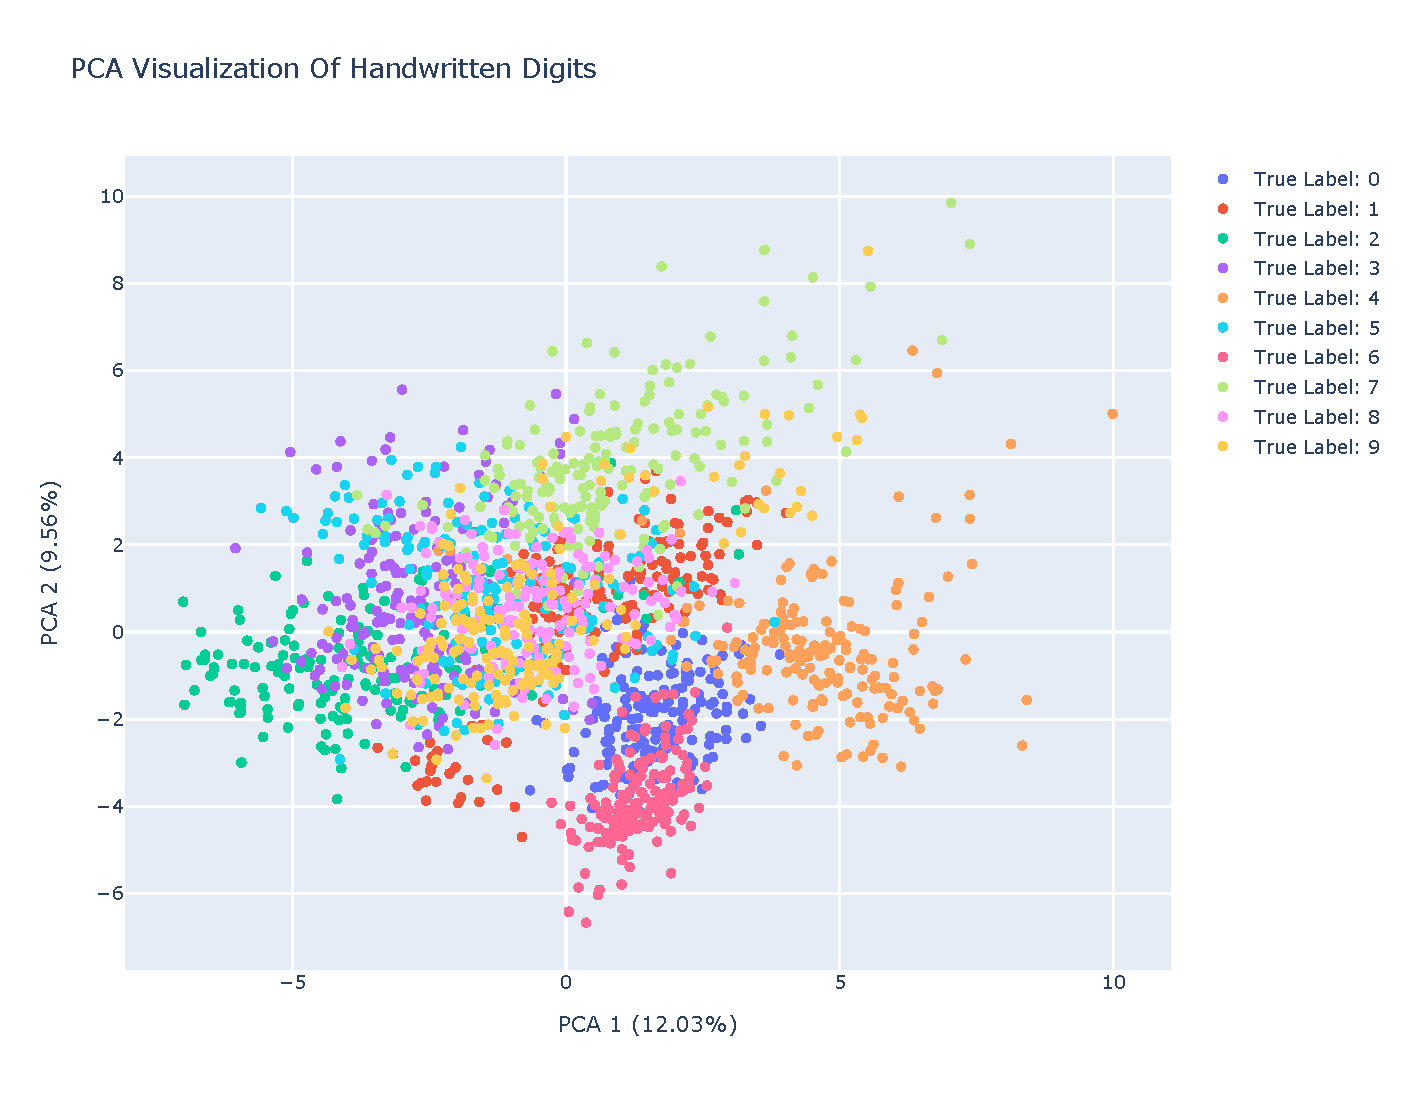
\includegraphics[width=\textwidth]{figures/digitspca}
    \caption{PCA visualization of handwritten digits.}%
    \label{fig:digitspca}
  \end{figure} 

  Unfortunately, individual clusters are hardly identifiable on this
  visualization as the top two components explain a very low variance ratio.
  The Handwritten Digits dataset being a non-trivial high-dimensional
  structure, this type of linear projections won't be able to perform well.
  Luckily, $t$-SNE, a popular visualization algorithm that is often very
  succesful at revealing clusters in data, can be used in this situation.
  $t$-SNE roughly works by trying to optimize for preserving the topology of
  the data. Figure~\ref{fig:digitstsne}, shows a $t$-SNE visualization of the
  dataset, projected on the top two components, obtained using
  Listing~\ref{lst:digitstsne}.

  \newpage

  \begin{lstlisting}[caption={Perform $t$-SNE and project on top two
  components.}, captionpos=b, label={lst:digitstsne}]
# Fit t-SNE with PCA initialization.
tsne = TSNE(n_components=2, init="pca", random_state=42)
X_tsne = tsne.fit_transform(X_norm)

fig = go.Figure()

for i in range(10):
  fig.add_trace(go.Scatter(
    x=X_tsne[y==i, 0],
    y=X_tsne[y==i, 1],
    mode="markers",
    marker_color=i,
    name="True Label: {}".format(i)
  ))

fig.update_layout(
  title="t-SNE Visualization Of Handwritten Digits",
  height=800
)
    
fig.show()
  \end{lstlisting}

  \begin{figure}[!ht]
    \centering
    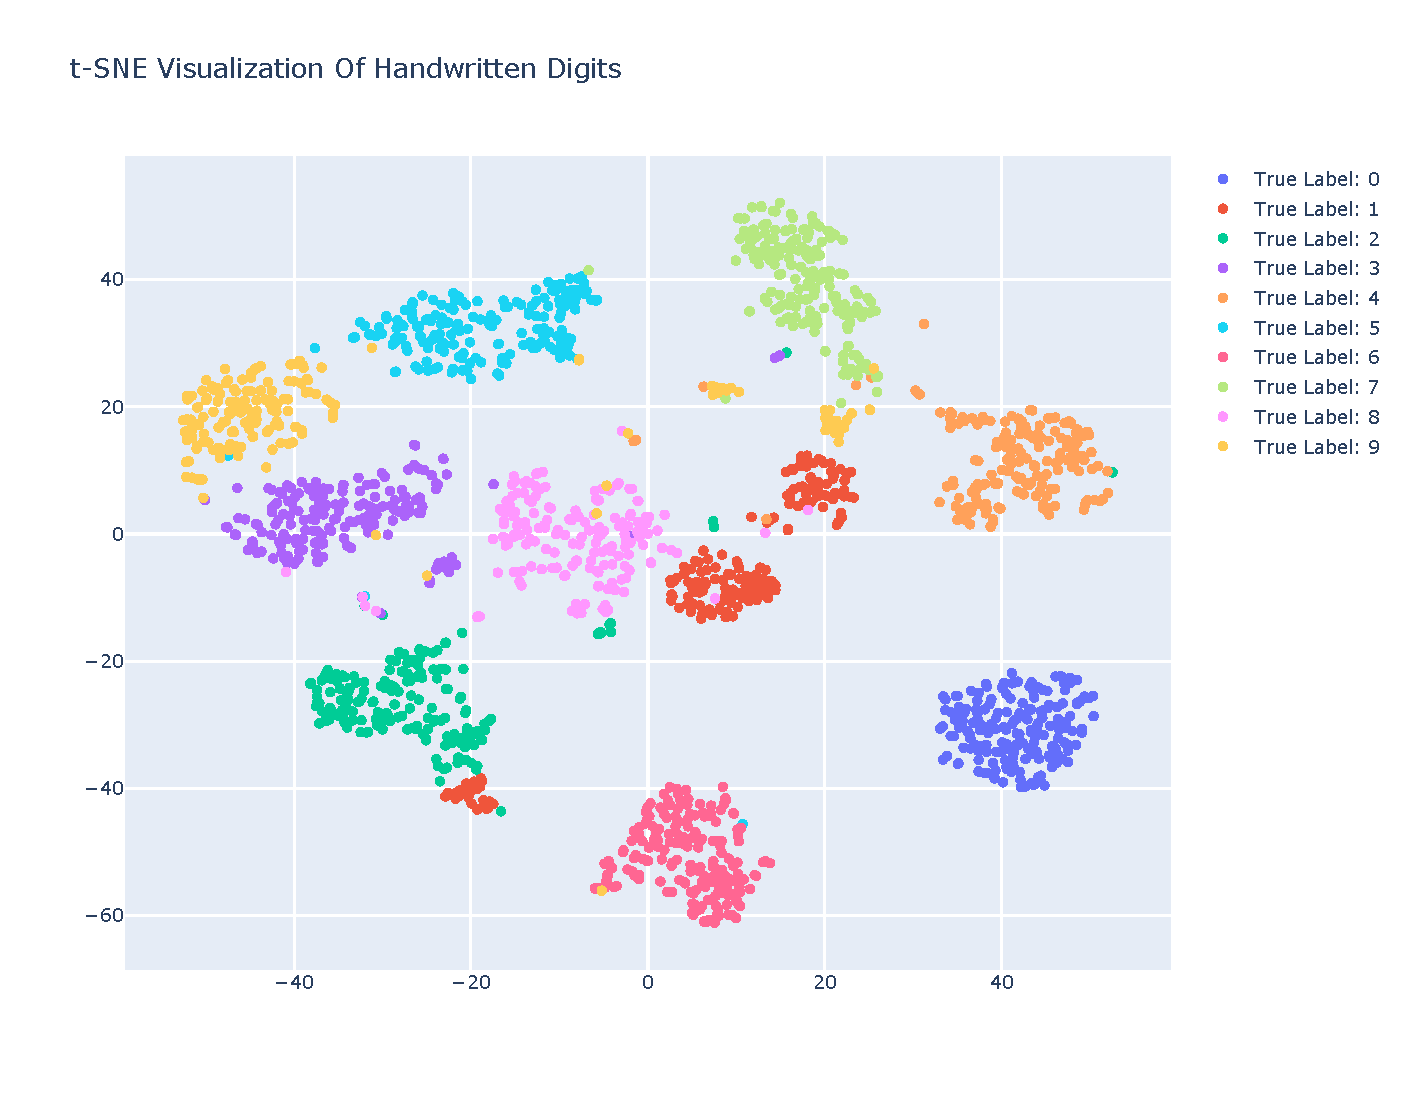
\includegraphics[width=\textwidth]{figures/digitstsne}
    \caption{$t$-SNE visualization of handwritten digits.}%
    \label{fig:digitstsne}
  \end{figure} 
\end{document}
